\chapter{Discrete methods in Image Processing}
\label{chapter:discrete-methods-in-image-processing}

\section{Markov Random Fields}

Let $G=(\mathcal{V},\mathcal{E})$ an undirected graph with vertices set $\mathcal{V}$ and edges set $\mathcal{E}$. The set of adjacent vertices to $v \in V$ is denoted $N(v)$. Given two subsets $S,Q \subset \mathcal{V}$, a $(S,Q)$-cut is any subset of edges $E' \subset E$ such that $S,Q$ are in different connected components in the graph $G(\mathcal{V},E \setminus E')$. We denote $cut(S,Q)$ the set of all $(S,Q)$ cuts.

For each vertex $v \in V$ we associate a discrete random variable $X_v$ that take values from a label set $\Lambda_v$ according with some distribution $P$. We group all variables in vector $\vec{X}$ and we write $X_S$ to refer to the set of associated variables with vertex set $S \subset \mathcal{V}$. We also group all the label sets in the collection $\Lambda$. We denote $\Omega$ the set of all configurations of the random variables. We say that the tuple $(G,\vec{X},\Lambda,P)$ forms a \emph{Markov Random Field} (MRF) if its probability distribution $P$  satisfies the independence conditions below

\begin{align}
	\textbf{Pairwise independencies:}&\quad \Big\{ X_v \perp X_u \;|\; \big\{X_i,\; i \neq u,v \big\}  \Big\} \label{ch2:eq:markov-pairwise-independencies}   \\
	\textbf{Local independencies:}&\quad \Big\{ X_v \perp X_u \;|\; \big\{X_i, \; i \notin \{v\}  \cup N(v)  \big\} \Big\} \label{ch2:eq:markov-local-independencies} \\
	\textbf{Global independencies:}& \quad \Big\{ X_S \perp X_Q \;|\; X_Z,\; \text{where } X_Z \in cut(S,Q) \Big\} \label{ch2:eq:markov-global-independencies},
\end{align}

\begin{figure}
\center
\begin{minipage}{0.3\textwidth}
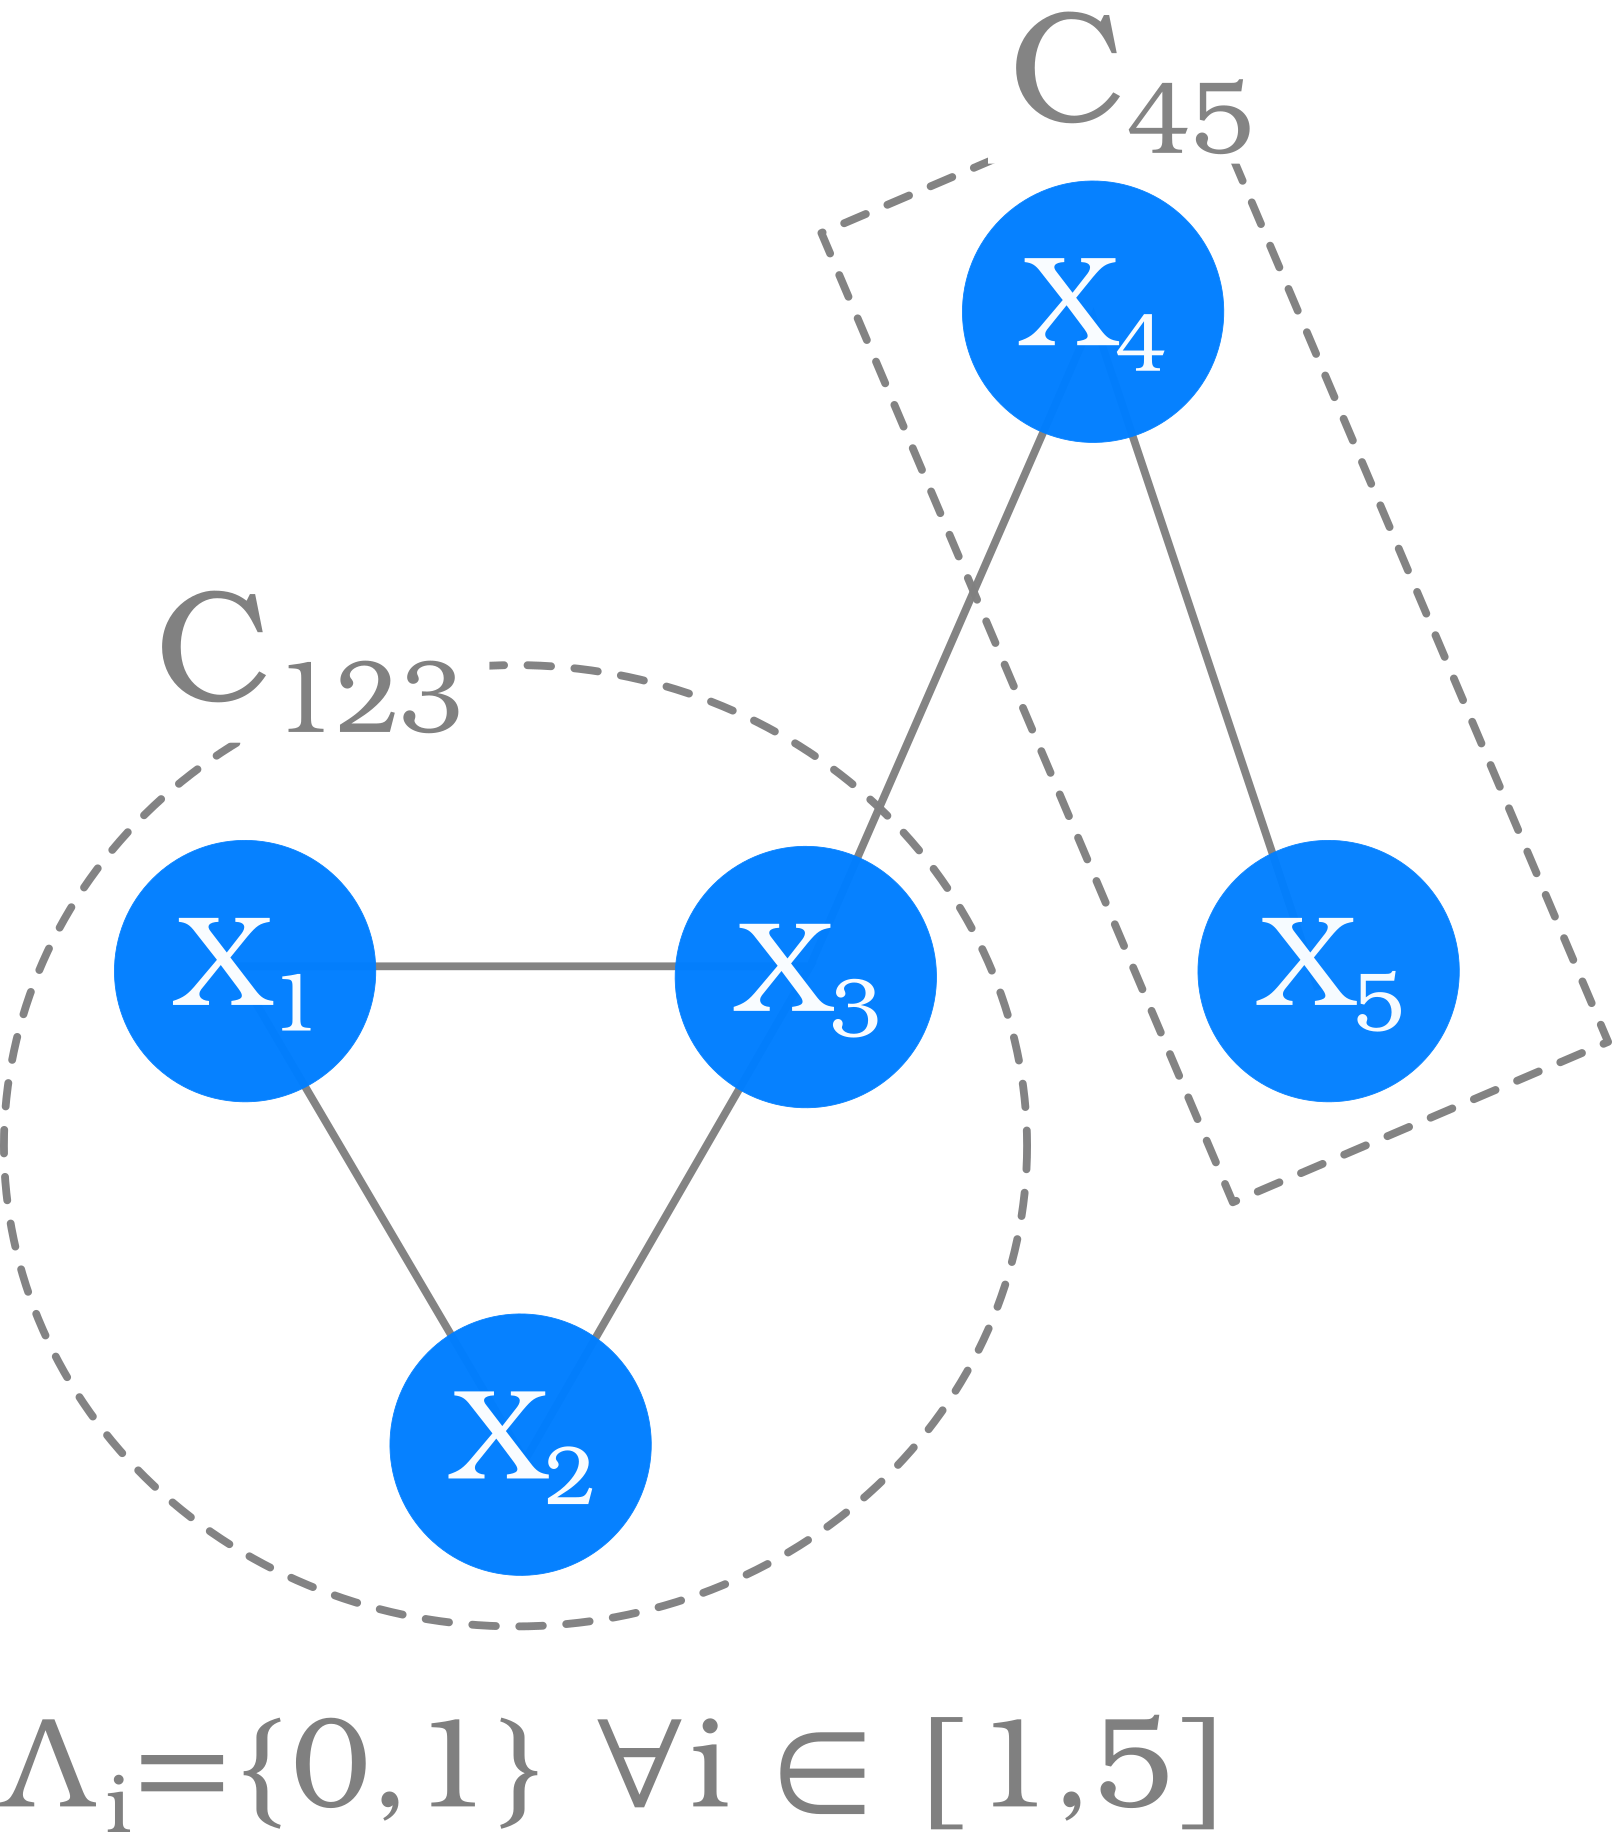
\includegraphics[scale=0.10]{figures/chapter3/mrf-example.png}
\end{minipage}%
\begin{minipage}{0.35\textwidth}
\tiny
\begin{tabular}{|c|c|c|c|c|l|}
\hline
\multicolumn{5}{|c|}{$\omega$} & \\
\hline
$X_1$ & $X_2$ & $X_3$ & $X_4$ & $X_5$ & $P(\omega)$\\
\hline
0 & 0 & 0 & 0 & 0 & 0.0238 \\
0 & 0 & 0 & 0 & 1 & 0.0023 \\
0 & 0 & 0 & 1 & 0 & 0.0011 \\
0 & 0 & 0 & 1 & 1 & 0.0059 \\
0 & 0 & 1 & 0 & 0 & 0.0238 \\
0 & 0 & 1 & 0 & 1 & 0.0023 \\
0 & 0 & 1 & 1 & 0 & 0.0011 \\
0 & 0 & 1 & 1 & 1 & 0.0059 \\
0 & 1 & 0 & 0 & 0 & 0.119 \\
0 & 1 & 0 & 0 & 1 & 0.0119 \\
0 & 1 & 0 & 1 & 0 & 0.0059 \\
0 & 1 & 0 & 1 & 1 & 0.0297 \\
0 & 1 & 1 & 0 & 0 & 0.0476 \\
0 & 1 & 1 & 0 & 1 & 0.0047 \\
0 & 1 & 1 & 1 & 0 & 0.0023 \\
0 & 1 & 1 & 1 & 1 & 0.0119 \\
\hline
\end{tabular}
\end{minipage}%
\begin{minipage}{0.35\textwidth}
\tiny
\begin{tabular}{|c|c|c|c|c|l|}
\hline
\multicolumn{5}{|c|}{$\omega$} &\\
\hline
$X_1$ & $X_2$ & $X_3$ & $X_4$ & $X_5$ & $P(\omega)$\\
\hline
1 & 0 & 0 & 0 & 0 & 0.119 \\
1 & 0 & 0 & 0 & 1 & 0.0119 \\
1 & 0 & 0 & 1 & 0 & 0.0059 \\
1 & 0 & 0 & 1 & 1 & 0.0297 \\
1 & 0 & 1 & 0 & 0 & 0.0476 \\
1 & 0 & 1 & 0 & 1 & 0.0047 \\
1 & 0 & 1 & 1 & 0 & 0.0023 \\
1 & 0 & 1 & 1 & 1 & 0.0119 \\
\textbf{1} & \textbf{1} & \textbf{0} & \textbf{0} & \textbf{0} & \textbf{0.238} \\
1 & 1 & 0 & 0 & 1 & 0.0238 \\
1 & 1 & 0 & 1 & 0 & 0.0119 \\
1 & 1 & 0 & 1 & 1 & 0.0595 \\
1 & 1 & 1 & 0 & 0 & 0.0952 \\
1 & 1 & 1 & 0 & 1 & 0.0095 \\
1 & 1 & 1 & 1 & 0 & 0.0047 \\
1 & 1 & 1 & 1 & 1 & 0.0238 \\
\hline
\end{tabular}
\end{minipage}
\caption{Example of a Markov Random Field. The nodes $X_1, X_2, X_3$ forms the $3$-clique $C_{123}$.}
\label{ch2:fig:example-mrf}
\end{figure}

where $X_v  \perp  X_u \;|\; X_S$ means that variable $X_v$ is independent of $X_u$ given variables in $X_S$.  For example, the MRF in~\cref{ch2:fig:example-mrf} respects the following expressions 

\begin{align*}
		P\Big(X_1=x_1 \; | \big\{X_i=x_i, \, i \neq 1 \big\} \Big) &= P\Big(X_1=x_1 \; | \; X_2=x_2,X_3=x_3 \Big) \\
		P\Big(X_3=x_3 \; | \big\{X_i=x_i, \, i \neq 3 \big\} \Big) &= P\Big(X_3=x_3 \; | \; X_1=x_1,X_2=x_2, X_4=x_4 \Big) \\
		P\Big(\vec{X}_{C_{123}} =\omega \; | \big\{X_i=x_i, \, i \notin \{1,2,3\}  \big\} \Big) &= P\Big(\vec{X}_{C_{123}} = \omega \; | \; X_4=x_4 \Big),		
\end{align*}

where we use the shorter notation $\vec{X}_{C_{123}} =\omega$ to denote some assignment of the random variables associated with the nodes of clique $C_{123}$. Given a graph, it may be quite difficult to sort out a probability distribution that satisfies~\cref{ch2:eq:markov-pairwise-independencies,ch2:eq:markov-local-independencies,ch2:eq:markov-global-independencies}. However, for the class of MRF that can be \emph{factorized} in terms of the maximal cliques of $G$, to create a valid probability distribution is straightforward with the help of \emph{clique potential} functions.

\subsubsection{Clique factorization and Gibbs distribution}

A distribution $P_{\Phi}$ is a \emph{Gibbs distribution} if it can be parameterized by a set of factors $\Phi = \{\phi_1,\phi_2,\dots \phi_m\}$, i.e., 

\begin{align*}
	P_{\Phi}(\omega) &= \frac{1}{Z}\prod_{i=1}^{m}{\phi(\omega)} \\
	Z &= \sum_{\omega \in \Omega}{ \prod_{i=1}^{m}{\phi(\omega)} }
\end{align*}


For strictly positive distributions ($P(\omega) > 0\; \forall \omega \in \Omega$), the \emph{Hammersley-Clifford} theorem states that $(G,\vec{X},\Lambda,P)$ is a MRF if and only if $P$ is a Gibbs distribution parameterized over complete subgraphs (clique) of $G$. Therefore, for MRF with strictly positive distributions $P$ we can write 

\begin{align*}
	P(w) &= \frac{1}{Z}\prod_{c \in \mathcal{C}}{\phi_c(w)} \\
	Z &=  \sum_{\omega \in \Omega}{ \prod_{c \in \mathcal{C}}{\phi_c(w)} },
\end{align*}

where $\mathcal{C}$ the set of all cliques of $G$. The MRF in~\cref{ch2:fig:example-mrf} was constructed by defining the following clique potentials

\begin{center}
\begin{tabular}{ccc}
\begin{tabular}{|c|c|c|c|}
\hline
$X_1$ & $X_2$ & $X_3$ & $\phi_{123}$\\
\hline
0 & 0 & 0 & 1\\
0 & 0 & 1 & 5\\
0 & 1 & 0 & 5\\
0 & 1 & 1 & 10\\
1 & 0 & 0 & 5\\
1 & 0 & 1 & 10\\
1 & 1 & 0 & 10\\
1 & 1 & 1 & 20\\
\hline
\end{tabular}&
\begin{tabular}{|c|c|c|}
\hline
$X_3$ & $X_4$ & $\phi_{34}$\\
\hline
0 & 0 & 100\\
0 & 1 & 50\\
1 & 0 & 20\\
1 & 1 & 10\\
\hline
\end{tabular}&
\begin{tabular}{|c|c|c|}
\hline
$X_4$ & $X_5$ & $\phi_{45}$\\
\hline
0 & 0 & 100\\
0 & 1 & 10\\
1 & 0 & 10\\
1 & 1 & 50\\
\hline
\end{tabular}
\end{tabular}
\end{center}

For strictly positive distributions we also have that the global independencies in~\cref{ch2:eq:markov-global-independencies} are equivalent to the pairwise and local independencies~\cite{koller09}.

\subsubsection{Grid graph and Tikhonov denoising revisited}
Let $I$ a grayscale bidemensional image with pixel coordinates $p=(p_x,p_y)$. We define its  undirected \emph{grid graph} $G_I(\mathcal{V},\mathcal{E})$ as

\begin{align*}
	\mathcal{V} &= \{ v_p \; | \; p \in I \} \\
	\mathcal{E} &= \big\{ \{v_p,v_u\} \; | \; p \in I[-1:-1] \text{ and } u + \{(1,0),(0,1)\}  \big\}
\end{align*}

In the grid graph $G_I$ we have $1$ and $2$-cliques only. To the grid graph of $I$ we construct the MRF $(G_I,\vec{X},\Lambda,P)$ in which the random variables take values over the grayscale levels of the image grouped in $\Lambda = \{i \; | \; 0 \leq i \leq 255 \}$ and the Gibbs distribution $P$ is of the form

\begin{align*}
	P(\omega) &= \frac{1}{Z}\prod_{u,v \in \mathcal{V} }{\phi_1(x_u)\phi_1(x_v)\phi_2(x_u,x_v)} \\
	Z &= \sum_{\omega \in \Omega}{ \prod_{u,v \in \mathcal{V} }{\phi_1(x_u)\phi_1(x_v)\phi_2(x_u,x_v)} },
\end{align*}

with clique potentials defined as

\begin{align*}
	\phi_1(u=\lambda _u) &= \exp\big( - \psi_1(\lambda_u) \big) \\
	\phi_2(u=\lambda _u,v=\lambda _v) &= \exp\big( - \psi_{12}(\lambda_u,\lambda_v) \big) \\[1em]
	\psi_{1}(\lambda_u) &=  \frac{1}{2} \left( f_{\widetilde{\vec{I}}}(u) - \lambda _u \right) ^2 \\
	\psi_{12}(\lambda_u, \lambda_v) &= \left\{ \begin{array}{ll} 
 ( \lambda _v - \lambda _u )^2, & v = u + (1,0) \text{ or } v = u + (0,1) \\
 \infty,& \text{otherwise}.
\end{array}\right.	
\end{align*}



In~\cref{ch2:fig:mrf-tikhonov-denoising} we have a representation of this MRF, which encodes the Tikhonov denoising model of~\cref{ch1:sec:bayesian-rationale}. The estimated image $\widehat{I}$ is computed as the maximum likelihood of $P$, i.e.,

\begin{align*}
	\widehat{\vec{I}} &= \argmax_{\vec{X}}{P(\vec{X}=\vec{I})} \\
	&= \argmin_{\vec{I}}{\sum_{u \in \Omega}{\psi_1\big({I(u)}\big)}} + \sum_{u,v \in \Omega}{\psi_{12}\big( {I(u),I(v) \big)}}.
\end{align*}

\begin{figure}
\center
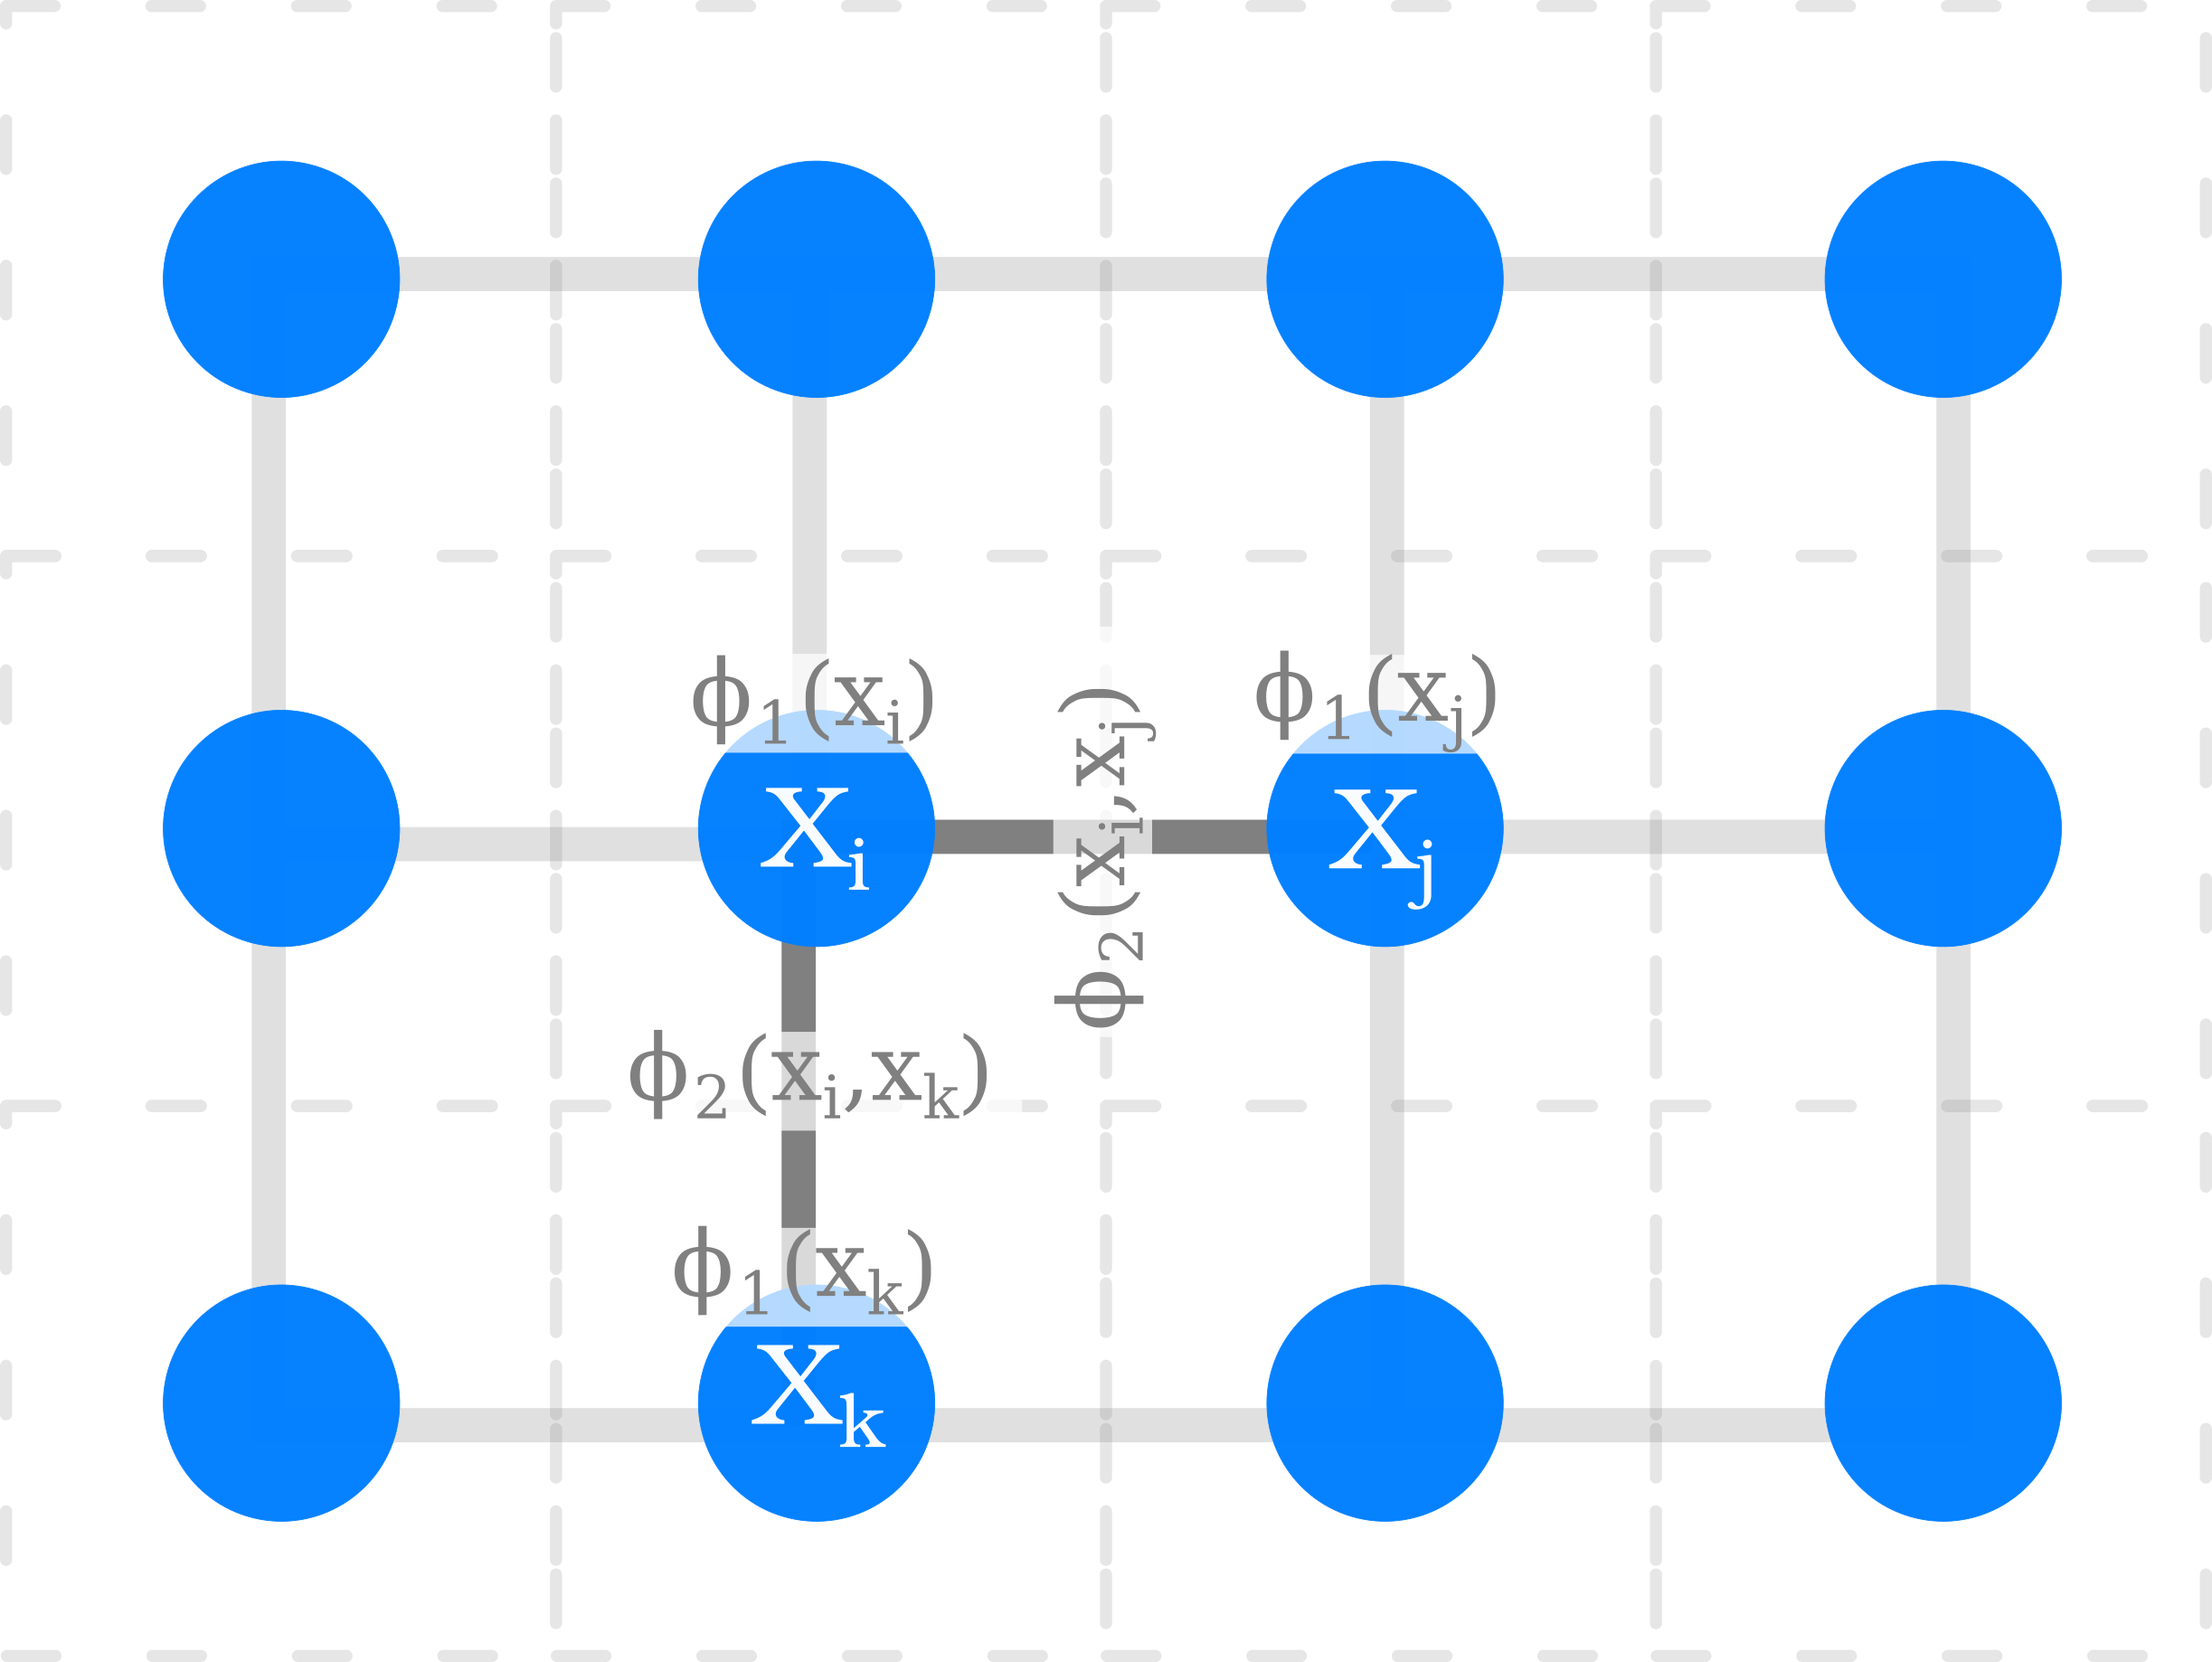
\includegraphics[scale=0.10]{figures/chapter3/grid-graph.png}
\caption{MRF illustration for Tikhonov image denoising}
\label{ch2:fig:mrf-tikhonov-denoising}
\end{figure}

\subsubsection{Hidden Markov model}

The model presented in the last section can be found with multiple flavors in the image processing literature in the context of multilabeling problems. We take the opportunity in this section to describe such model in its general form.

\begin{definition}{Hidden Markov Model}
A Hidden Markov Model is a MRF $(G,\vec{X} \cup \vec{Y}, \Lambda_X \cup \Lambda_Y,P)$ such that

\begin{align*}
	Y &= \{ Y_i \; | \; X_i \in \vec{X} \} \\
	\forall i \neq j,& \quad Y_i \perp X_j \; | \; X_i \\
	\forall i \neq j,& \quad Y_i \perp Y_j	.
\end{align*}
\end{definition}

We are going to be interested in problems arising from the setting in which the states of random variables in $\vec{Y}$ are known, and one wishes to infer the states of random variables in $\vec{X}$. In other words, we are interest to find $\vec{X}^{\star}$ such that

\begin{align}
	\vec{X}^{\star} &= \argmax_{\vec{X}} = P(\vec{X} \; | \; \vec{Y}) \nonumber \\
	&= \argmin_{\vec{X}}{ \sum_{c \in \mathcal{C}}{\phi_c(\vec{X})}}.
	\label{ch2:eq:general-maximum-likelihood}
\end{align}

\begin{figure}
\center
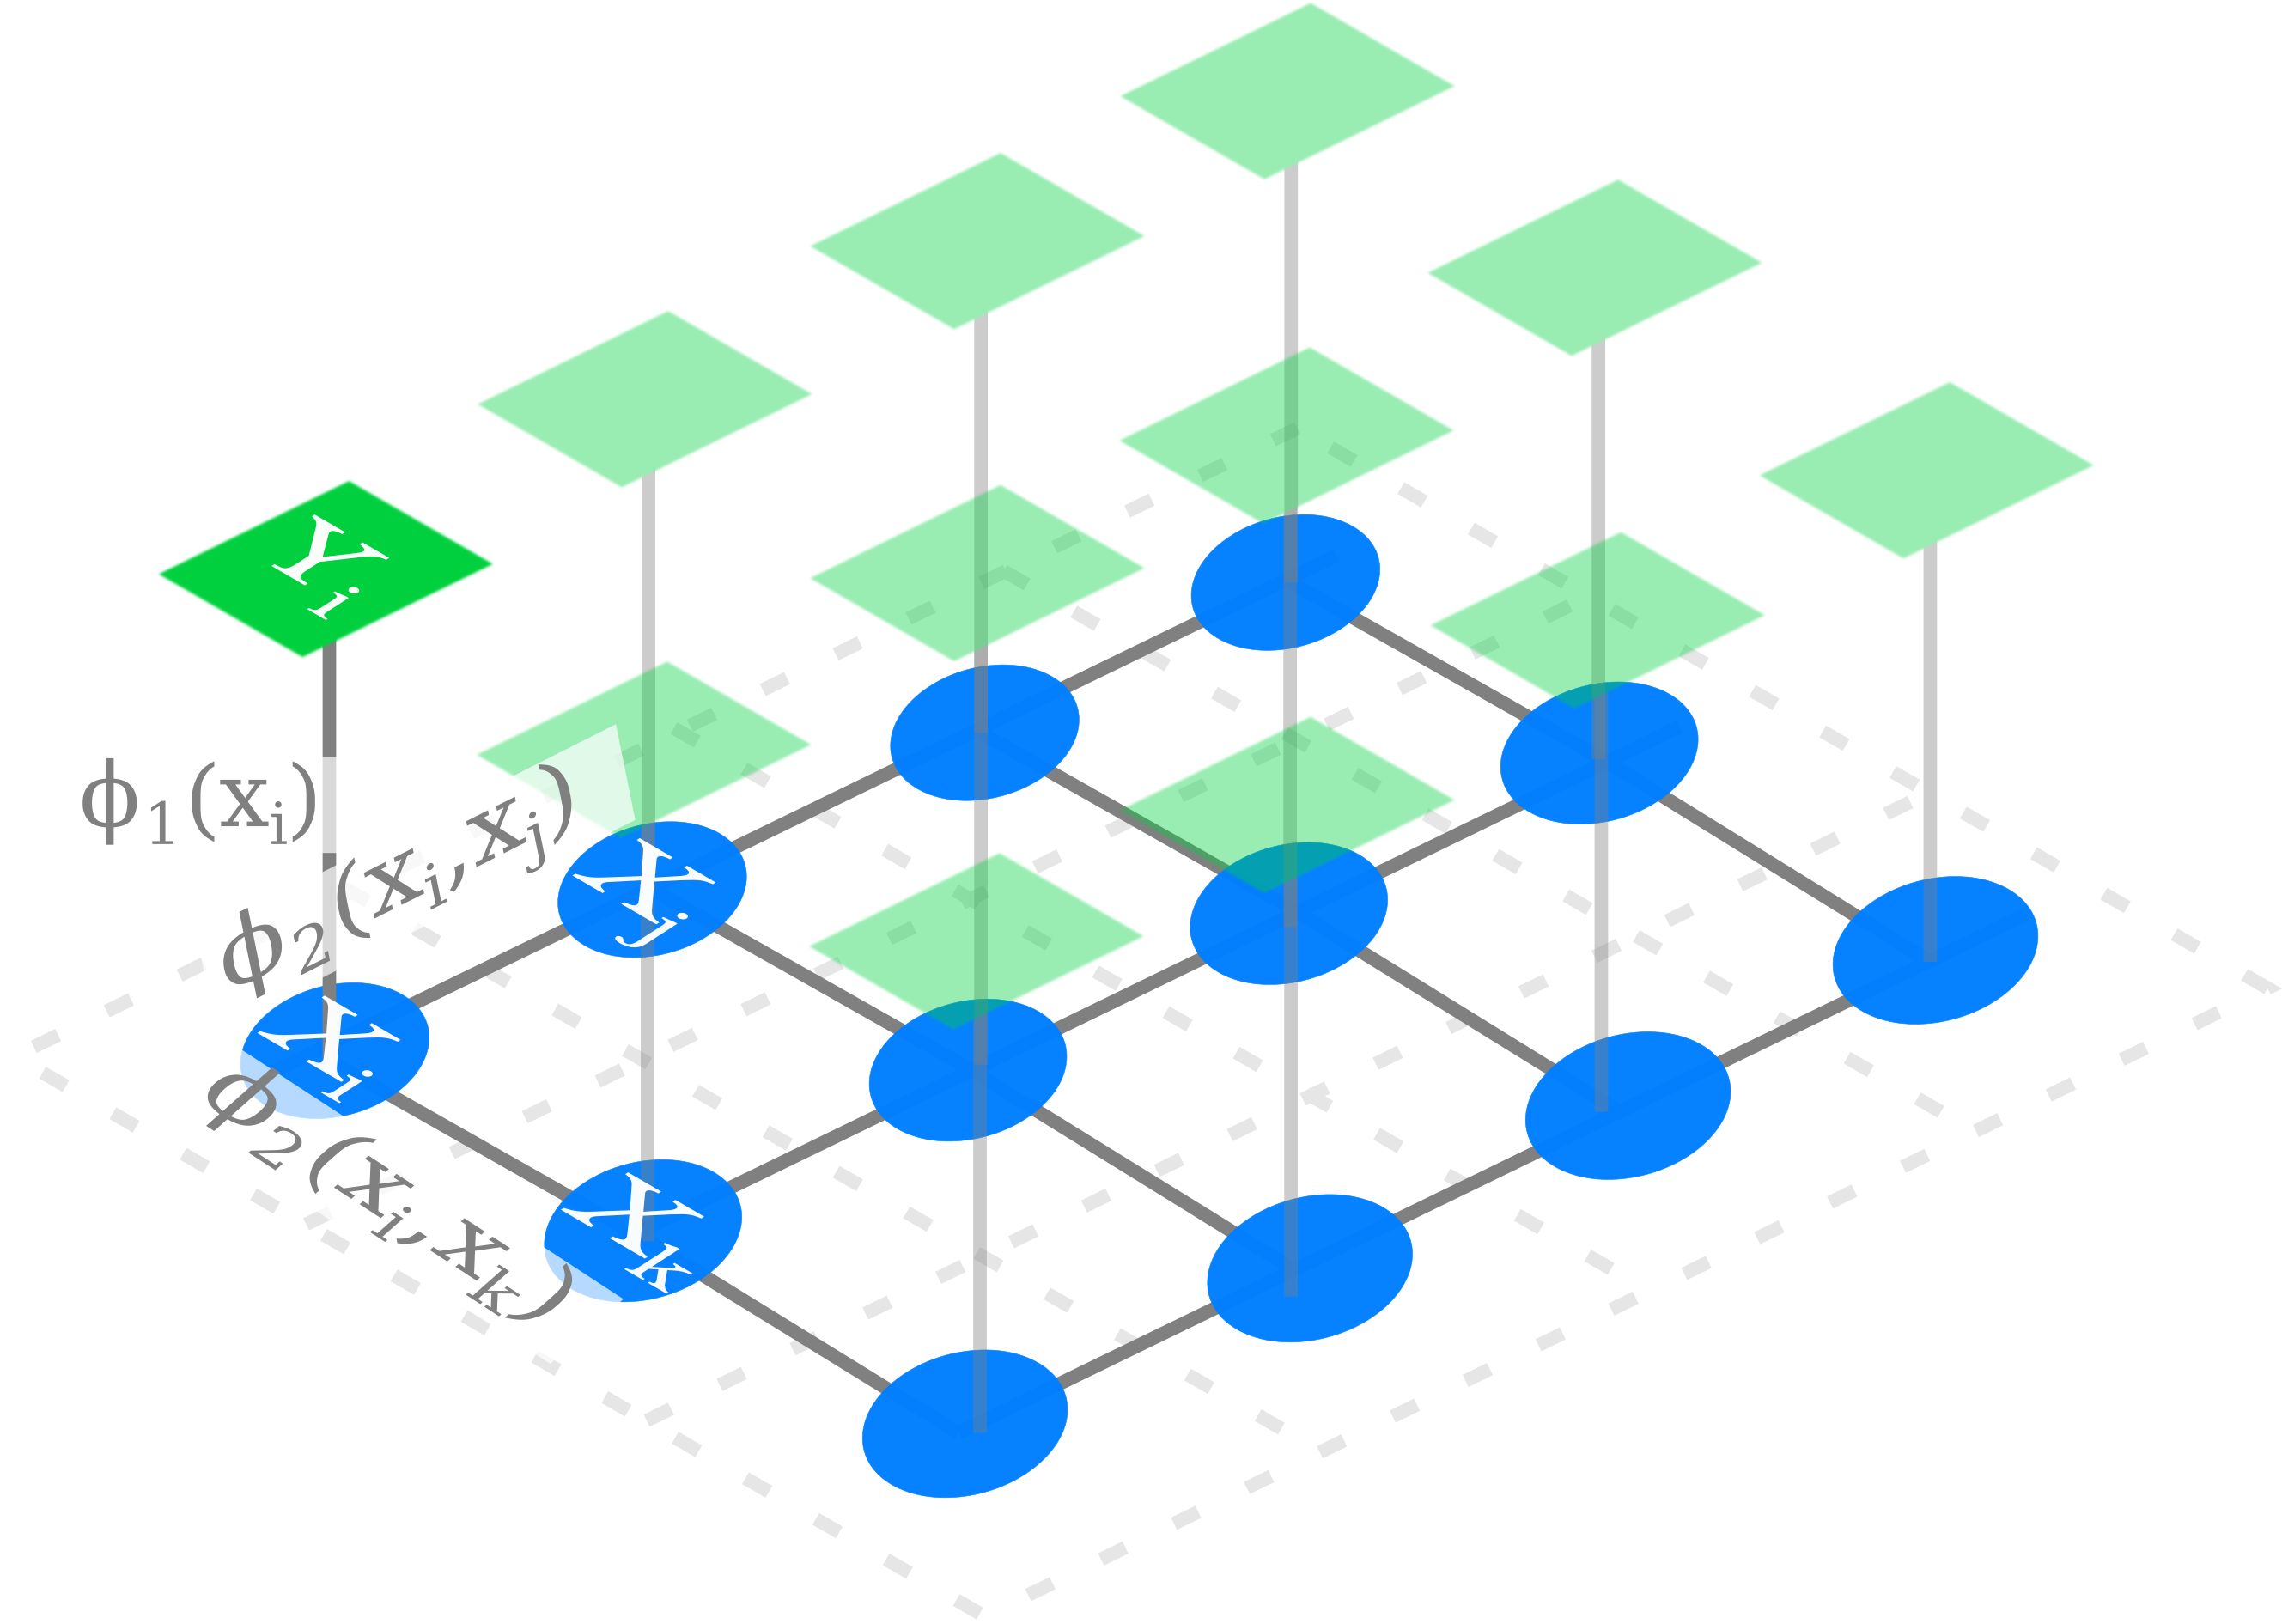
\includegraphics[scale=0.10]{figures/chapter3/hmm-example.png}
\caption{General $4$-adjacency HMM for multilabeling image problems}
\label{ch2:fig:hmm-multilabeling}
\end{figure}

 The variables $\vec{Y}$ are called observable states, and in image problems they are usually associated to the color intensity of the corresponding pixel. 

The set of labels $\Lambda_X$ is defined according to the problem. In segmentation it could mean the different partitions in which to segment the image. We could have a label that encodes the grass, another to encode the sky and so on. In stereo, the labels could mean the relative depth of the object with respect the others. In denoising and reconstruction problems in general, it could be the color intensities itself. The graph representation for the HMM of the Tikhonov denoising model looks like the graph in~\cref{ch2:fig:hmm-multilabeling}.

The success of this approach depends on our capacity to optimize~\cref{ch2:eq:general-maximum-likelihood}. Let's first observe that a multilabel MRF can always be transformed into an equivalent binary MRF~\cite{ishikawa10}. Therefore, we can restrict our analysis to binary MRFs.

In binary MRFs, the clique potentials maps binary vectors to real values, i.e., the clique potentials are \emph{pseudo-boolean} functions. It can be shown that any pseudo-boolean function can be transformed into an equivalent quadratic pseudo-boolean function~\cite{boros02pseudo}, in which each term involves at most two binary variables. Therefore, to optimize~\cref{ch2:eq:general-maximum-likelihood} it is sufficient to know how to optimize expressions of type

\begin{align*}
	\sum_{j}{f_j(x_j)} + \sum_{j<k}{f_{j,k}(x_k)}.
\end{align*} 

In the next section, we explore the class of pseudo-boolean functions and how we can optimize them.

\sketch{It is missing to talk about the Ising and Potts model in this section}

\section{Pseudo-boolean functions}

\begin{definition}{Pseudo-boolean function}
	A pseudo boolean function $f:\{0,1\}^n \rightarrow \mathbb{R}$ is a function that maps binary vectors to real values.
\end{definition}

Pseudo-boolean functions (PBF) can be interpreted as \emph{set functions}, i.e., functions that map sets to real values. Indeed, a binary vector of $n$ elements is in bijection with the power sets of $V = \{1,2,\cdots,n\}$. Therefore, the PBF $f:\{0,1\}^n \rightarrow \mathbb{R}$ can be written as

\begin{align}
	f(x_1,\cdots,x_n) &= \sum_{S \subset 2^{V}}{c_S \prod_{i \in S}{x_i}}.
	\label{ch2:eq:pbf-polynomial-form}
\end{align}

where $c_S \in \mathbb{R}$ is a coefficient associated to each subset $S$. ~\cref{ch2:eq:pbf-polynomial-form} is denoted the \emph{polynomial form} of PBF $f$. The \emph{order} of a PBF is defined as the cardinality of the largest subset $S$ in which $c_S>0$. The polynomial form is unique. 

Sometimes is convenient to express $f$ in its so called \emph{posiform} representation, usually denoted by $\phi$ instead of $f$. In its posiform representation we use literals $x_i,\bar{x}_i \in L$  to represent states $1,0$ of indexed variable $i$ and all coefficients are positive except the one associated to the empty set.

\begin{align}
	\phi(f) = \phi(x_1,\cdots,x_n) &= \sum_{T \subset 2^{L}}a_T{\prod_{p \in T}{p}},
\end{align}

where $a_T \geq 0$ whenever $T\neq \emptyset$. The posiform representation can be seen as a truth table with positive values for all configurations, except the one in which all variables are set to zero. One can pass from posiform to polynome representation by exchanging $\bar{x}_i$ and $(1-x_i)$. A posiform is said \emph{maximum-constant}  if its constant term $C(\phi)$ is maximum among all posiforms representing $f$. A maximum-constant posiform is denoted $\phi^{\star}$. Both general and maximum-constants posiforms are not unique representations of the PBF $f$.

\begin{example}The polynomial form and two possible posiform representations for the same PBF.
\begin{align*}
	f(x_1,x_2) &= a_{\emptyset} + a_\ol{1} + a_\ol{2} + a_\ol{12} + \big(a_1 - a_\ol{1} + a_{1\ol{2}} - a_\ol{12}\big)x_1 \\
	&+ \big(a_{2} - a_\ol{2} + a_{\ol{1}2} - a_{\ol{12}}\big)x_2\\ 
	&+ \big(a_{12} - a_{\ol{1}2} - a_{1\ol{2}} + a_{\ol{12}}\big)x_1x_2 \\[1em]
	\phi_1(x_1,x_2) &= a_{\emptyset} + a_1x_1 + a_\ol{1}\ol{x_1} + a_2x_2 + a_\ol{2}\ol{x_2} \\ 
			&+ a_{12}x_1x_2 + a_{\ol{1}2}\ol{x_1}x_2 + a_{1\ol{2}}x_1\ol{x_2} + a_{\ol{12}}x_1\ol{x_2} \\[1em]			
	\phi_2(x_1,x_2) &= (a_{\emptyset}-c) + (a_1+c)x_1 + (a_\ol{1}+c)\ol{x_1} + a_2x_2 + a_\ol{2}\ol{x_2} \\ 
			&+ a_{12}x_1x_2 + a_{\ol{1}2}\ol{x_1}x_2 + a_{1\ol{2}}x_1\ol{x_2} + a_{\ol{12}}x_1\ol{x_2} 	
\end{align*}
\end{example}

Classical problems in combinatorial optimization as vertex cover, maximum independent set, $3$-SAT and many others are formulated as PBF optimization problems. The mentioned problems are in NP-complete, so we can expect that the optimization of a general PBF is a task that is unlikely to be solved efficiently. Nonetheless, we can investigate subclasses of PBF in which the optimum can be found in a reasonable time.

\subsubsection{PBF optimization}
 We first observe that optimizing a PBF of order $n$ can be transformed into an equivalent quadratic PBF optimization problem by creating extra variables and penalty terms. For example, let $x,y,w,z \in \{0,1\}$. Then,
 
 \begin{align*}
 	z=xy \leftrightarrow  xy -2xz-2yz+3x=0 \\
 	z \neq xy \leftrightarrow  xy -2xz-2yz+3x>0
 \end{align*}
 
 Therefore
 
\begin{align*}
	\min f(x,y,w) &= \min g(x,y,w,z) \\
    \min xyw &= \min zw + xy -2xy -2yz +3x .
\end{align*} 

  This procedure can be extended and formally described in a polynomial time algorithm that transforms an arbitrary PBF $f$ in a quadratic PBF $g$ with the property that $\min f = \min g$~\cite{boros02pseudo}. Therefore, we can limit the analysis to the optimization of quadratic PBFs.
  
\subsubsection{Roof duality}

A quite natural and naive approach to optimize~\cref{ch2:eq:pbf-polynomial-form} would be to formulate the quadratic PBF as a continuous linear programming. Consider the quadratic PBF

\begin{align}
	F(\vec{x}) = \left\{ \begin{array}{rl}
		\min &c_0 + \sum_{}{c_ix_i} + \sum_{}{c_{ij}x_ix_j} \\
	\text{subject to }& \vec{x} \in \{0,1\}^n.
	\end{array}\right.
	\label{ch2:eq:qpbf-qip-formulation}
\end{align}

~\cref{ch2:eq:qpbf-qip-formulation} can be linearized by substituting each pairwise term $x_ix_j$ with binary variable $z_{ij}$ and including the following set of constraints 

\begin{align*}
	C(\vec{x},\vec{z}) &= \left\{  \begin{array}{l}
	z_{ij} \leq x_i, \\
	z_{ij} \leq x_j, \\
	z_{ij} \geq x_i + x_j - 1 
	\end{array} \Bigg|\; \forall 0<i<j<n \right\}
\end{align*}

Therefore, an equivalent linear integer programming formulation is

\begin{align}
	\begin{array}{rl}
		\min& c_0 + \sum_{}{c_ix_i} + \sum_{}{c_{ij}z_{ij}} \\
		\text{subject to }&  \vec{x},\vec{z} \in \{0,1\}^n\\
		&C(\vec{x},\vec{z})	
	\end{array}
	\label{ch2:eq:qpbf-lp-formulation}
\end{align}

Finally, the relaxation of~\cref{ch2:eq:qpbf-lp-formulation} gives

\begin{align*}
	G(\vec{x},\vec{z}) &= \left\{ \begin{array}{rl}
		\min& c_0 + \sum_{}{c_ix_i} + \sum_{}{c_{ij}z_{ij}} \\
		\text{subject to }&  \vec{x},\vec{z} \in [0,1]^n\\
		&C(\vec{x},\vec{z})
	\end{array}\right.
\end{align*}

Clearly, formulation $G$ is a lower bound of $F$, i.e.,  $G(\vec{x},\vec{z}) \leq F(\vec{x})$. Such lower bound is called the \emph{roof dual} (it was originally defined for a maximization problem) and its shown~\cite{hammer84} to be equivalent to

\begin{align*}
	G(\vec{x},\vec{z}) &= C_{\phi^{\star}(f)}
\end{align*}

In this same work, the so called \emph{strong persistency} theorem is proven. It says that for every unary term $a_uu$ ($u$ a literal) in a max-constant posiform representation of $f$, we have that $u=0$ in every solution of $\min f$.

\begin{example}
Consider the quadratic PBF 
\begin{align*}
	f(x_1,x_2,x_3) &= 6-x_1-4x_2-x_3+3x_1x_2+x_2x_3.
\end{align*}

It can be shown that its roof dual equals $2$. A possible max-constant posiform representation for $f$ is

\begin{align*}
	\phi^{\star}(f) &= 2 + x_1 + \bar{x}_2 + x_1x_2 +2\bar{x}_1\bar{x}_2 + \bar{x}_2\bar{x}_3
\end{align*}

According with the strong persistency theorem, $x_1=0,\bar{x}_2=0$ for every solution of $\min f$. Replacing this values in $f$ we have

\begin{align*}
	\min f(x_1,x_2,x_3) &=\min f(x_1=0,\bar{x}_2=0,x_3) \\
	&= \min 6 - 4 - x_3 + x_3 \\
	&= 2.
\end{align*}
\end{example}

The strong persistency theorem allow us to fix some variables of the quadratic PBF, which could possibly result in a simpler optimization problem. Clearly, the main difficult is to find the max-constant posiform $\phi^{\star}(f)$ that results in a maximum number of variable elimination. Such posiform, called the \emph{master posiform}, can be found by finding the maximum flow in a capacitated graph.

\subsubsection{Master posiform and max-flow reduction}

We proceed by giving a construction of a capacitated graph $G(\mathcal{V},\mathcal{E},c)$ that encodes some posiform $\phi$ with constant $C(\phi)=0$. Let $\phi$ be a posiform of the form
	\begin{align*}
		\phi &= \sum_{p \in L}{a_pp} + \sum_{p,q \in L}{a_{pq}pq},
	\end{align*}
	
with $a_p >0, a_{pq}>0\; \forall p,q \in L$	. We  construct the capacitated graph $G_{\phi}(\mathcal{V},\mathcal{E},c)$ such that each term in the sum is encoded by two edges. Each unary term with literal $p$ have one edge from the source to its negated literal vertex $v_{\bar{p}}$ and one edge from $v_p$ to the target vertex. Pairwise terms with literals $p,q$ have edges $(v_p,v_{\bar{q}})$ and $(v_q,v_{\bar{p}})$.

\begin{align*}
	\mathcal{V} =& \{ v_p \; | \; p \in L \} \cup \{s,t\} \\[1em]
	\mathcal{E} =& \big\{ (s, v_{\bar{p}}),(v_p,t) \; | \; \forall a_p>0 \big\} \cup \big\{ (v_p,v_{\bar{q}} ), (v_q,v_{\bar{p}} ) \; | \; \forall a_{vq} > 0 \big\}  \\[1em]
	c(\, (v_p,v_q)\, ) = c_{pq} =& \left\{ \begin{array}{rl}
		a_{p}/2, & \text{if } v_p \notin \{s,t\} \text{ or } v_q \notin \{s,t\} \\
		a_{pq}/2, & \text{if } v_p,v_q \notin \{s,t\}\\ 
		0,& \text{otherwise}.
	\end{array}\right.
\end{align*}

A construction of graph $G_{\phi}$ is illustrated in~\cref{ch2:fig:posiform-capacitated-graph-a}. Therefore, the posiform $\phi$ can also be written as $\phi = \sum_{(v_p,v_q) \in \mathcal{E}}{ c_{p\bar{q}} }$. In fact, it is possible to shown that there is a bijection between the posiform with zero constant $\phi$ and the graph $G_{\phi}$.


A flow is a function $\varphi:\mathcal{E}\rightarrow \mathbb{R}_{+}$ that satisfies

\begin{equation*}
	\begin{array}{rll}
	\varphi(\,(v_p,v_q)\,) = \varphi (p,q) <& c_{pq},&  \forall v_p,v_q \in \mathcal{V} \\[1em]
	\sum_{v_p \in \mathcal{V}}{\varphi(p,q)} =& \sum_{v_p \in \mathcal{V}}{\varphi (q,p)}, & \forall v_q \in \mathcal{V}.	
	\end{array}
\end{equation*}

A flow $\varphi ^{\star}$ is said to be maximum if 
\begin{align*}
	\varphi ^{\star} &= \argmax_{\varphi} \sum_{v_p \in \mathcal{V}}{\varphi(s,v_p)},
\end{align*}

i.e., if the flow leaving the source is maximum. The residual graph of $G_{\phi}$ with respect to some flow $\varphi$ is denoted $G_{ \phi [ \varphi ] }(\mathcal{V},\mathcal{E}^+,r)$ and owns the same set of vertices of $G_{\phi}$. The set of edges is extended to include returning edges as well, i.e.,

\begin{align*}
	\mathcal{E}^+ &= \mathcal{E} \cup \{ (v_q,v_p) \; | \; (v_p,v_q) \in \mathcal{E} \}.
\end{align*}

The edges cost is given by the residual function $r$

\begin{align*}
	r(\, (v_p,v_q)\, ) = r_{pq} &= \left\{ \begin{array}{ll}
	c_{pq} - \varphi( p,q ), & (v_p,v_q) \in \mathcal{E}\\
	\varphi( p,q ), & (v_p,v_q) \in \mathcal{E}^+ \setminus \mathcal{E}.
\end{array}\right.	 
\end{align*}

One can also construct a posiform from the residual graph $G_{ \phi [ \varphi ] }$. In this case, the posiform is denoted $\phi_{G_{ \phi [ \varphi ] }}$. We remark that edges arriving in the source or leaving the target are all mapped to $0$, as the source and the target are identified with the constants $1,0$ respectively. For example, $(p,s)$ is encoded as $p\bar{s}=0$.

The \emph{Ford-Fulkerson} algorithm computes the maximum flow by incrementing an initial zero flow function $\varphi_0=0$ every time an \emph{augmenting path} is found. The $k$-th augmenting path is a path $\pi_k = (p_0=s,p_1,p_2,\cdots,p_n,p_{n+1}=t)$ in the residual graph $G_{ \phi [\varphi_{t-1}] }$ in which all edges of $\pi_k$ have a positive residual value. We say that $\pi_k$ is an $\epsilon$-augmenting path if 

\begin{align*}
	\epsilon = \min_{p,q \in \pi_k} r_{p,q}.
\end{align*}

\begin{figure}
\center
\subfloat[Initial graph $G_{\phi}$ for $\phi = 2x + 8z + 2x\bar{z} + 4\bar{x}y + 6\bar{y}\bar{z}$\label{ch2:fig:posiform-capacitated-graph-a}]{
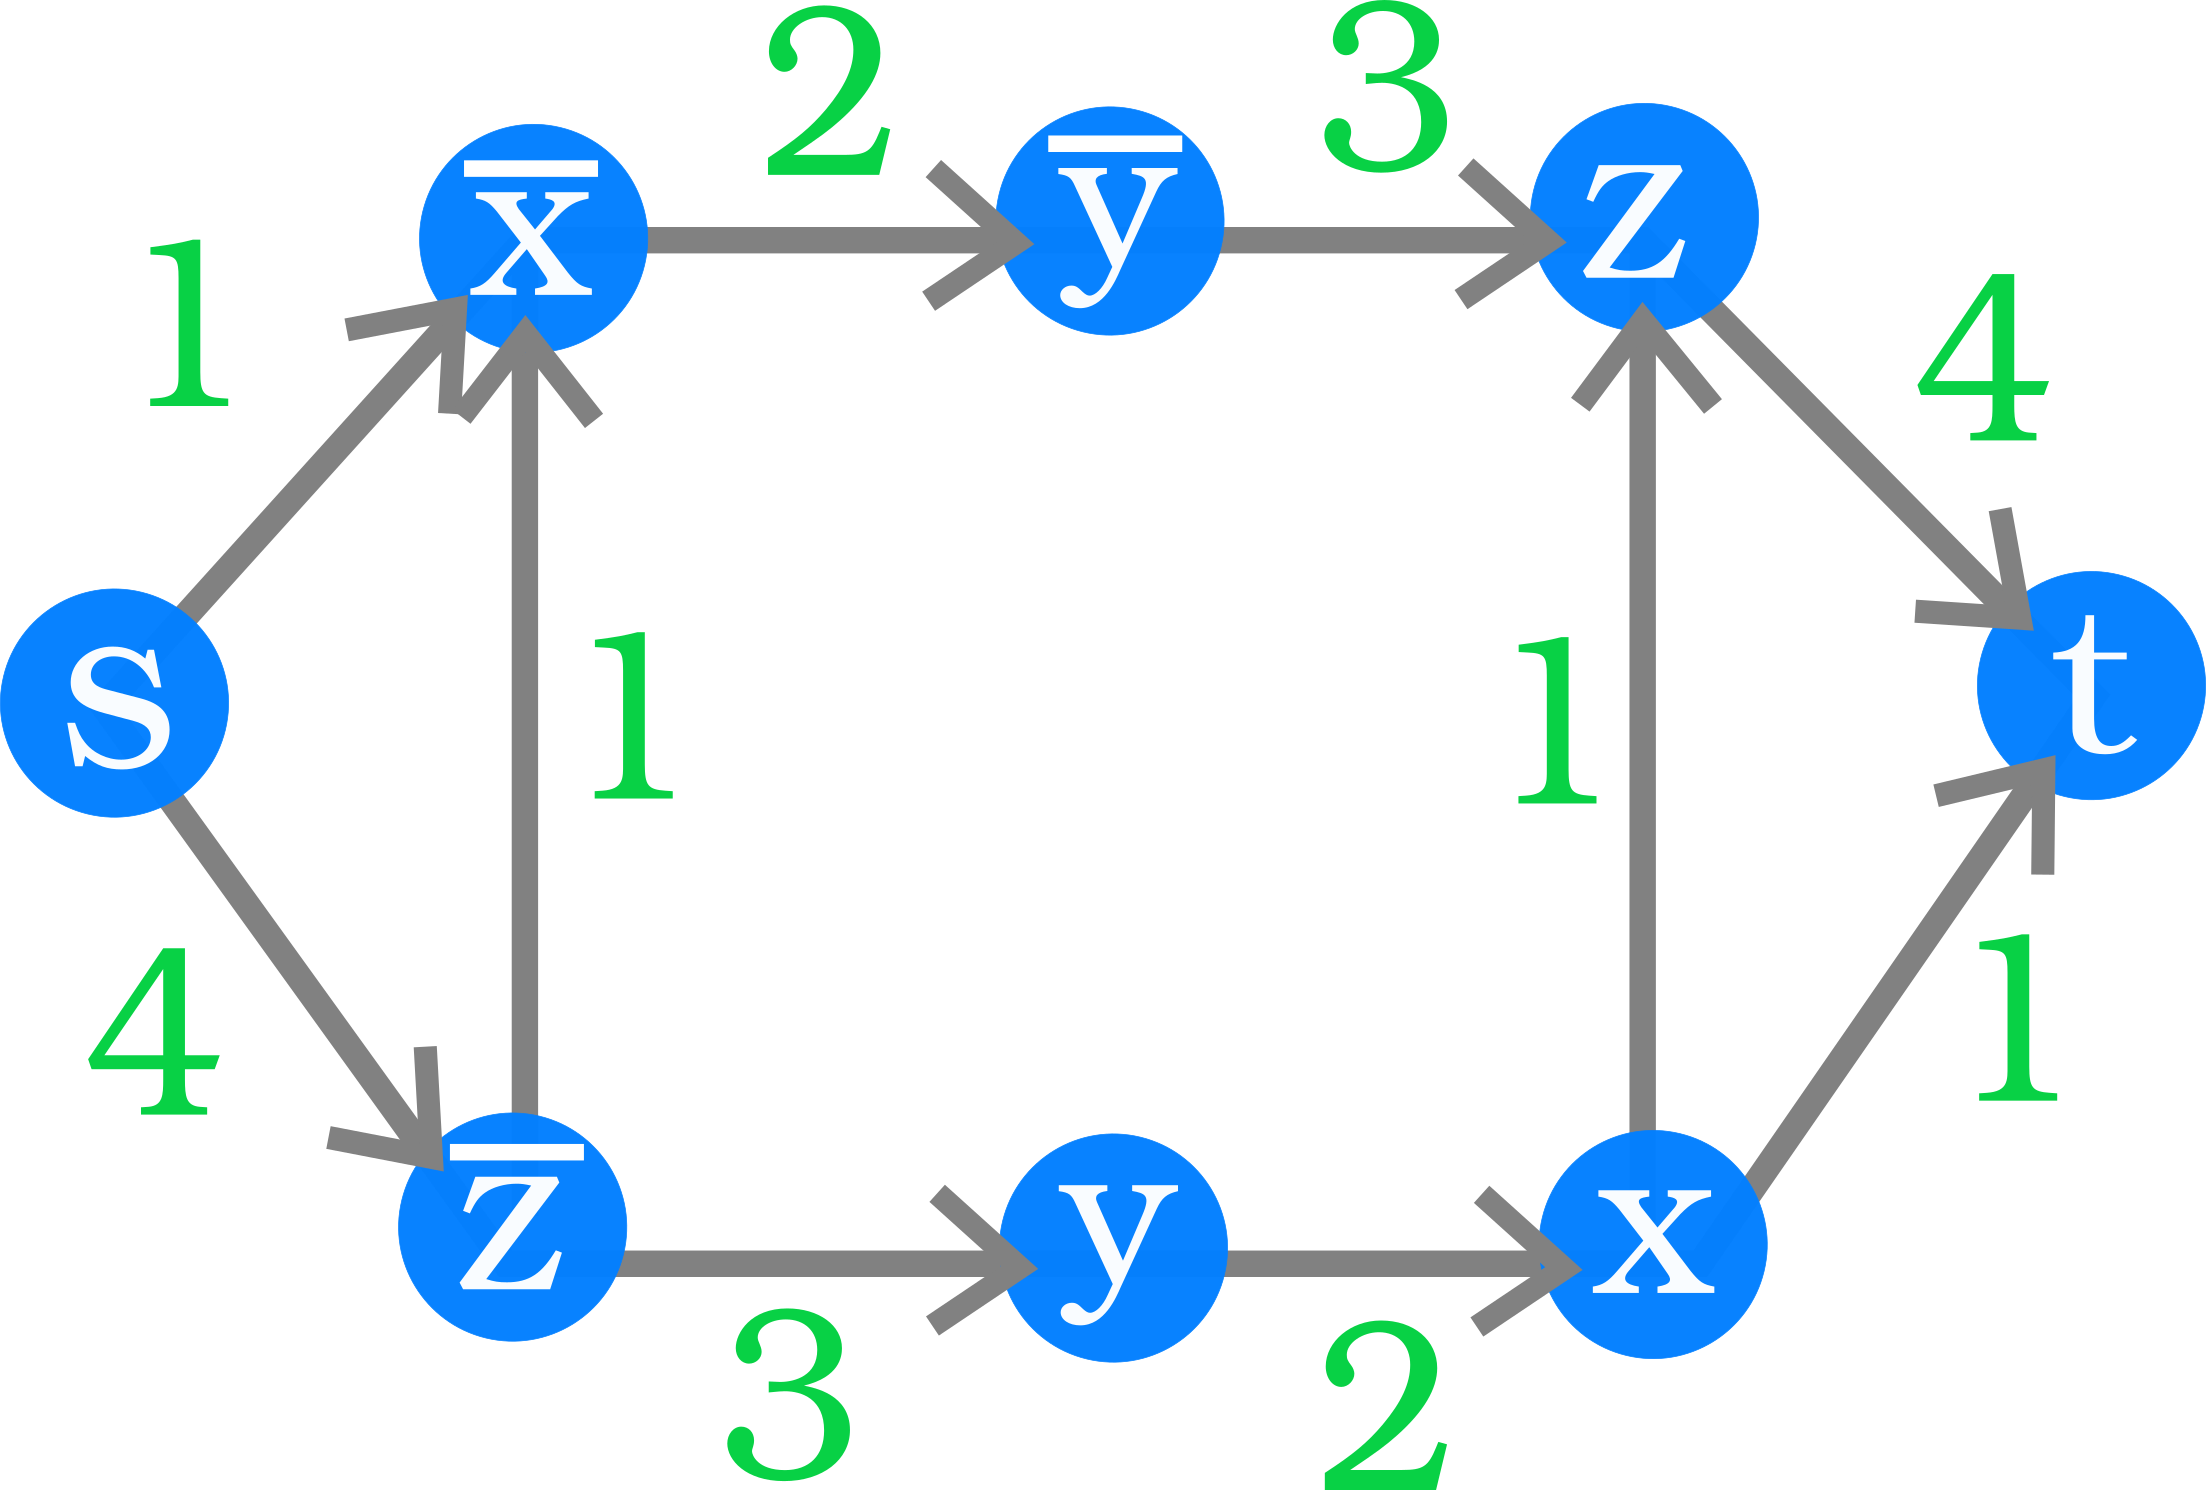
\includegraphics[scale=0.1]{figures/chapter3/posiform-graph-1.png}
}\\
\subfloat[Augmenting path $1$]{
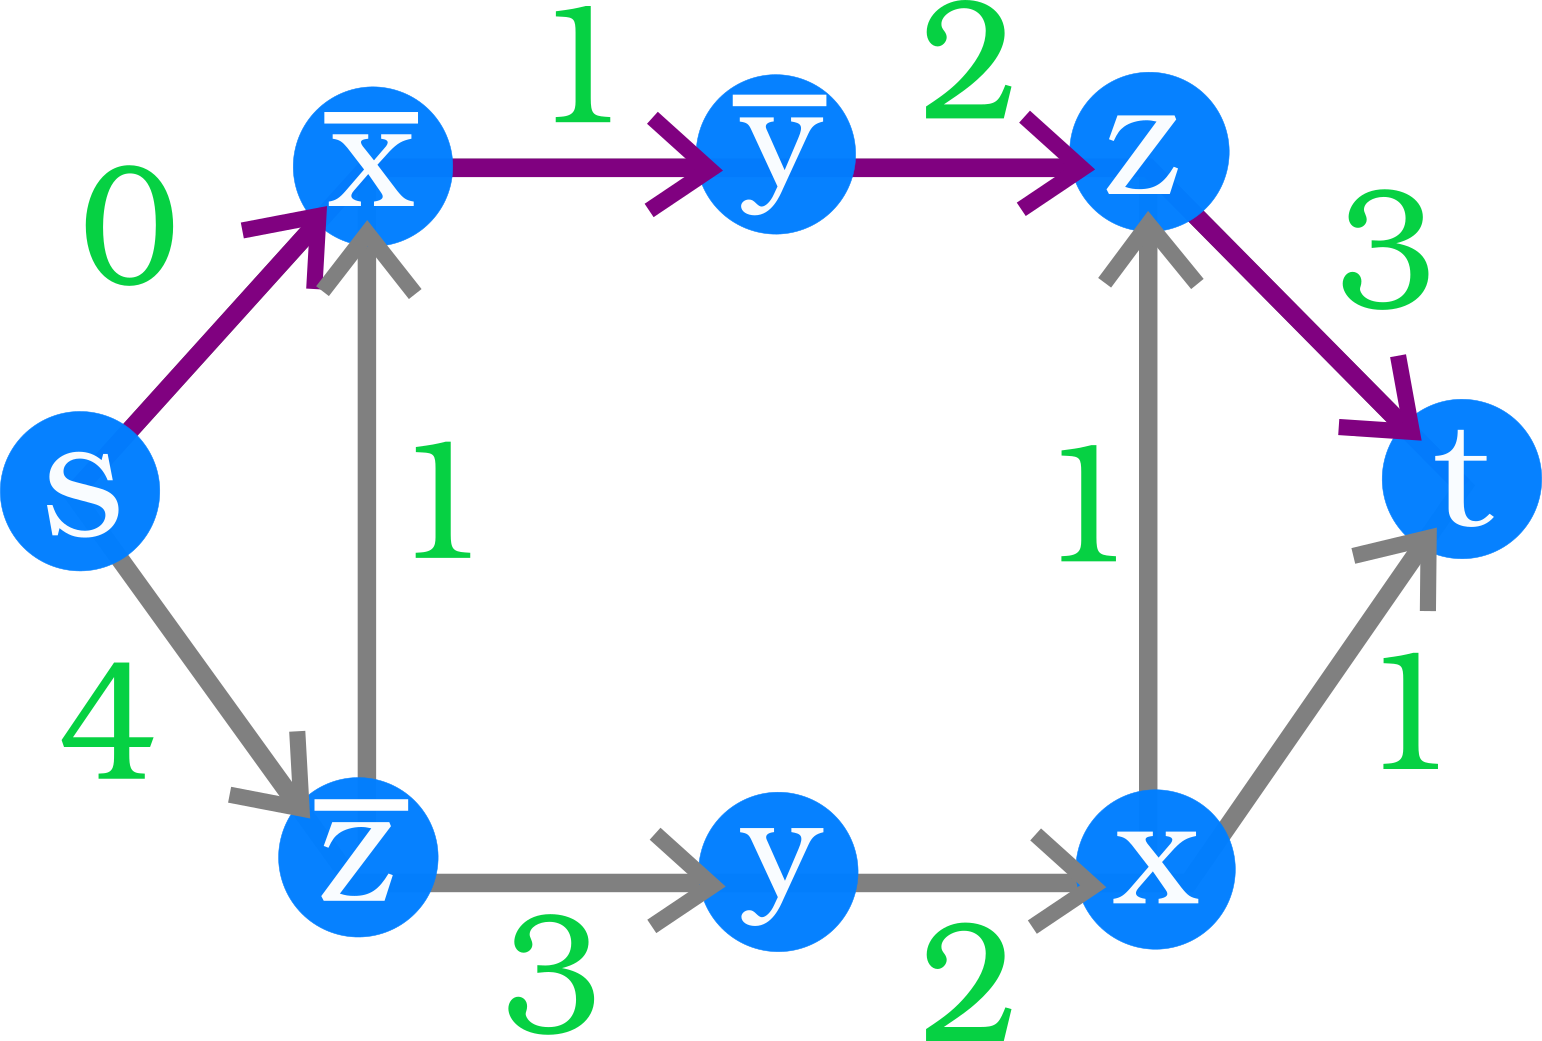
\includegraphics[scale=0.1]{figures/chapter3/posiform-graph-2.png}
}%
\subfloat[Augmenting path $2$]{
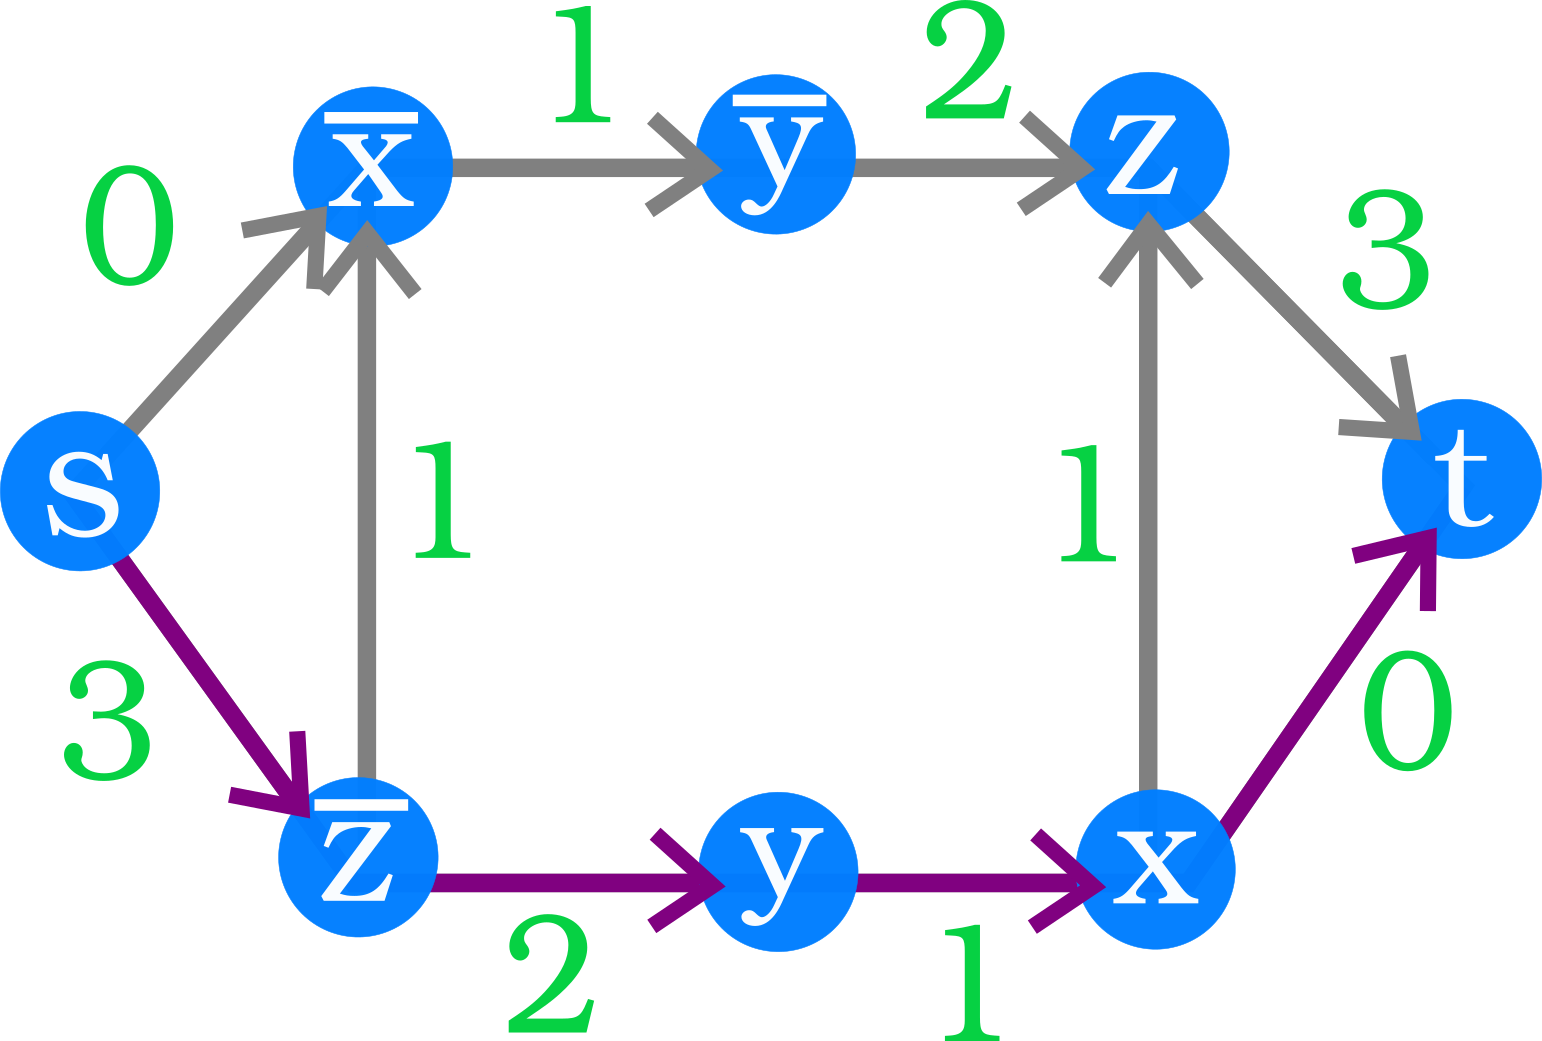
\includegraphics[scale=0.1]{figures/chapter3/posiform-graph-3.png}
}\\%
\subfloat[Augmenting path $3$]{
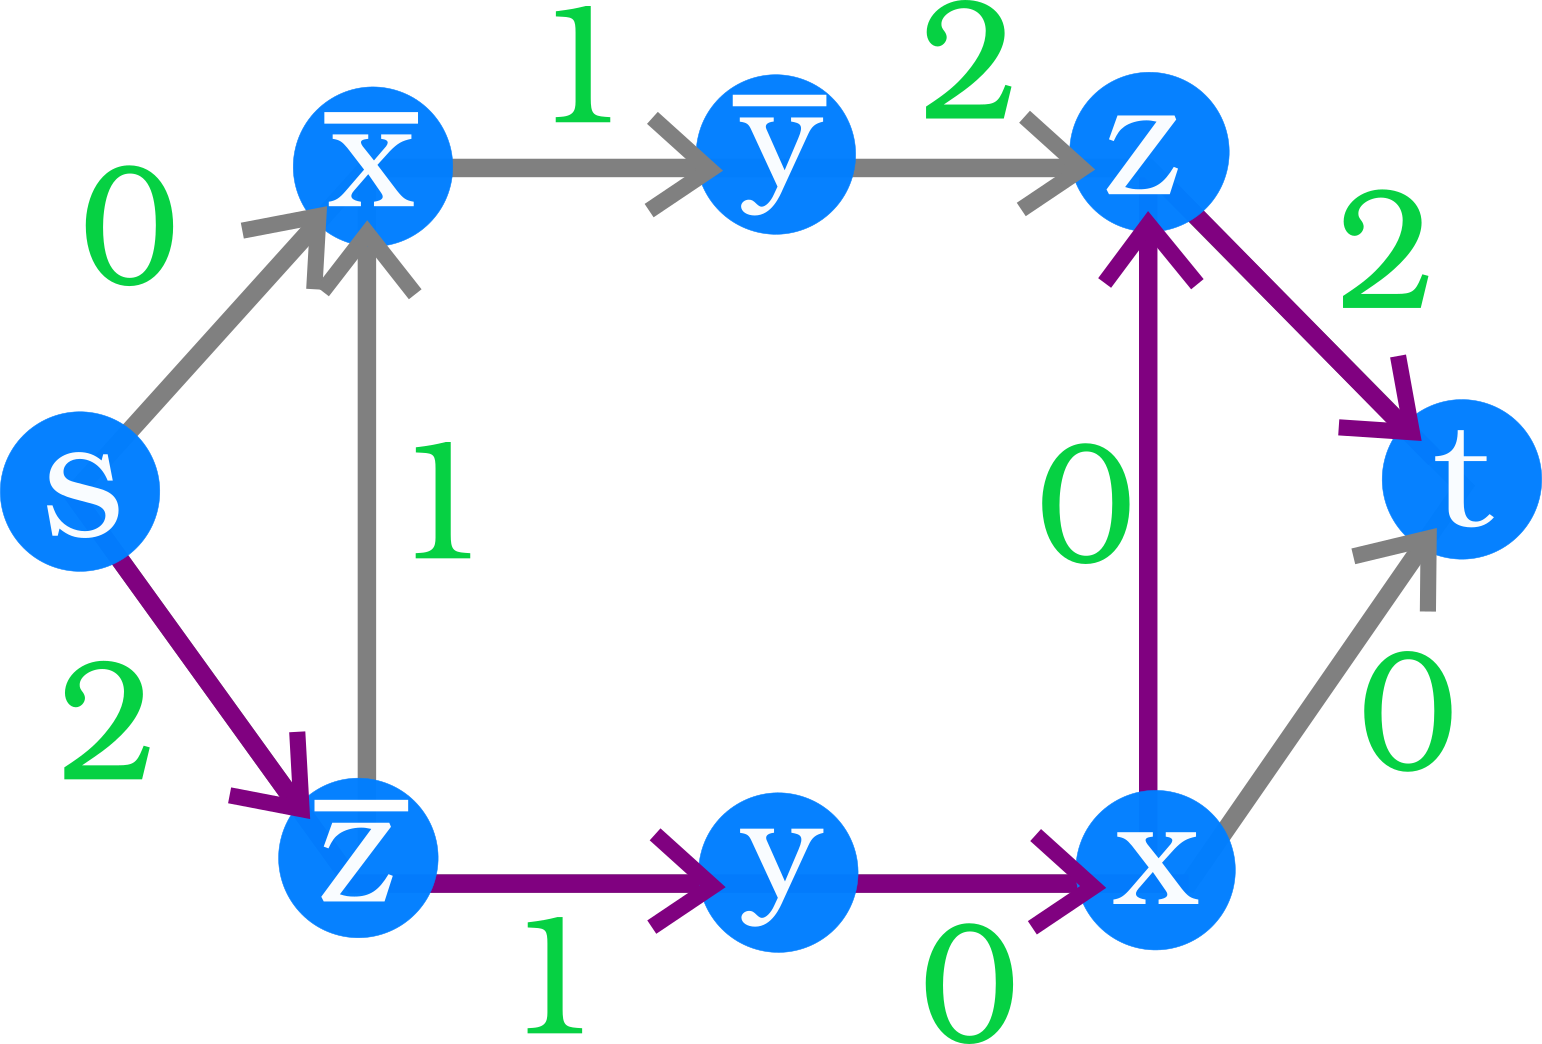
\includegraphics[scale=0.1]{figures/chapter3/posiform-graph-4.png}
}%
\subfloat[Augmenting path $4$]{
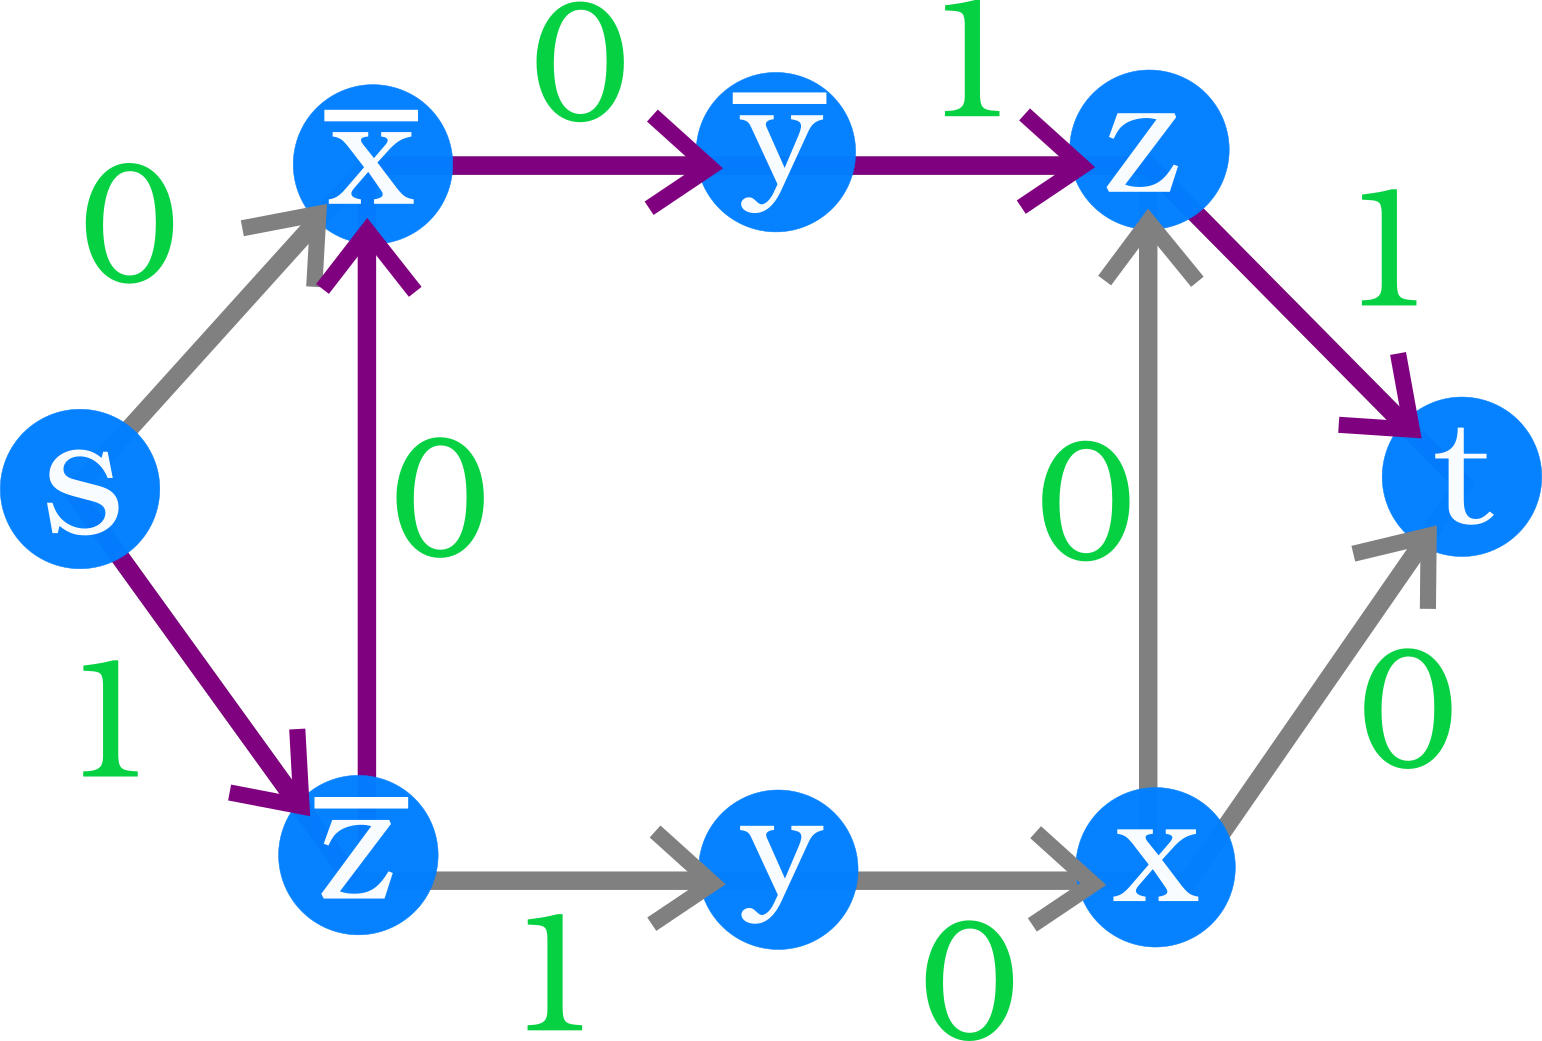
\includegraphics[scale=0.1]{figures/chapter3/posiform-graph-5.png}
}\\%
\subfloat[Final residual graph $G_{ \phi {[\varphi^{\star}]} }$. The master posiform is written as $ { \phi^{\star} } = 4 + 2z +2\bar{z}\bar{y} + 4zy + 4\bar{y}x + 2z\bar{x}$]{
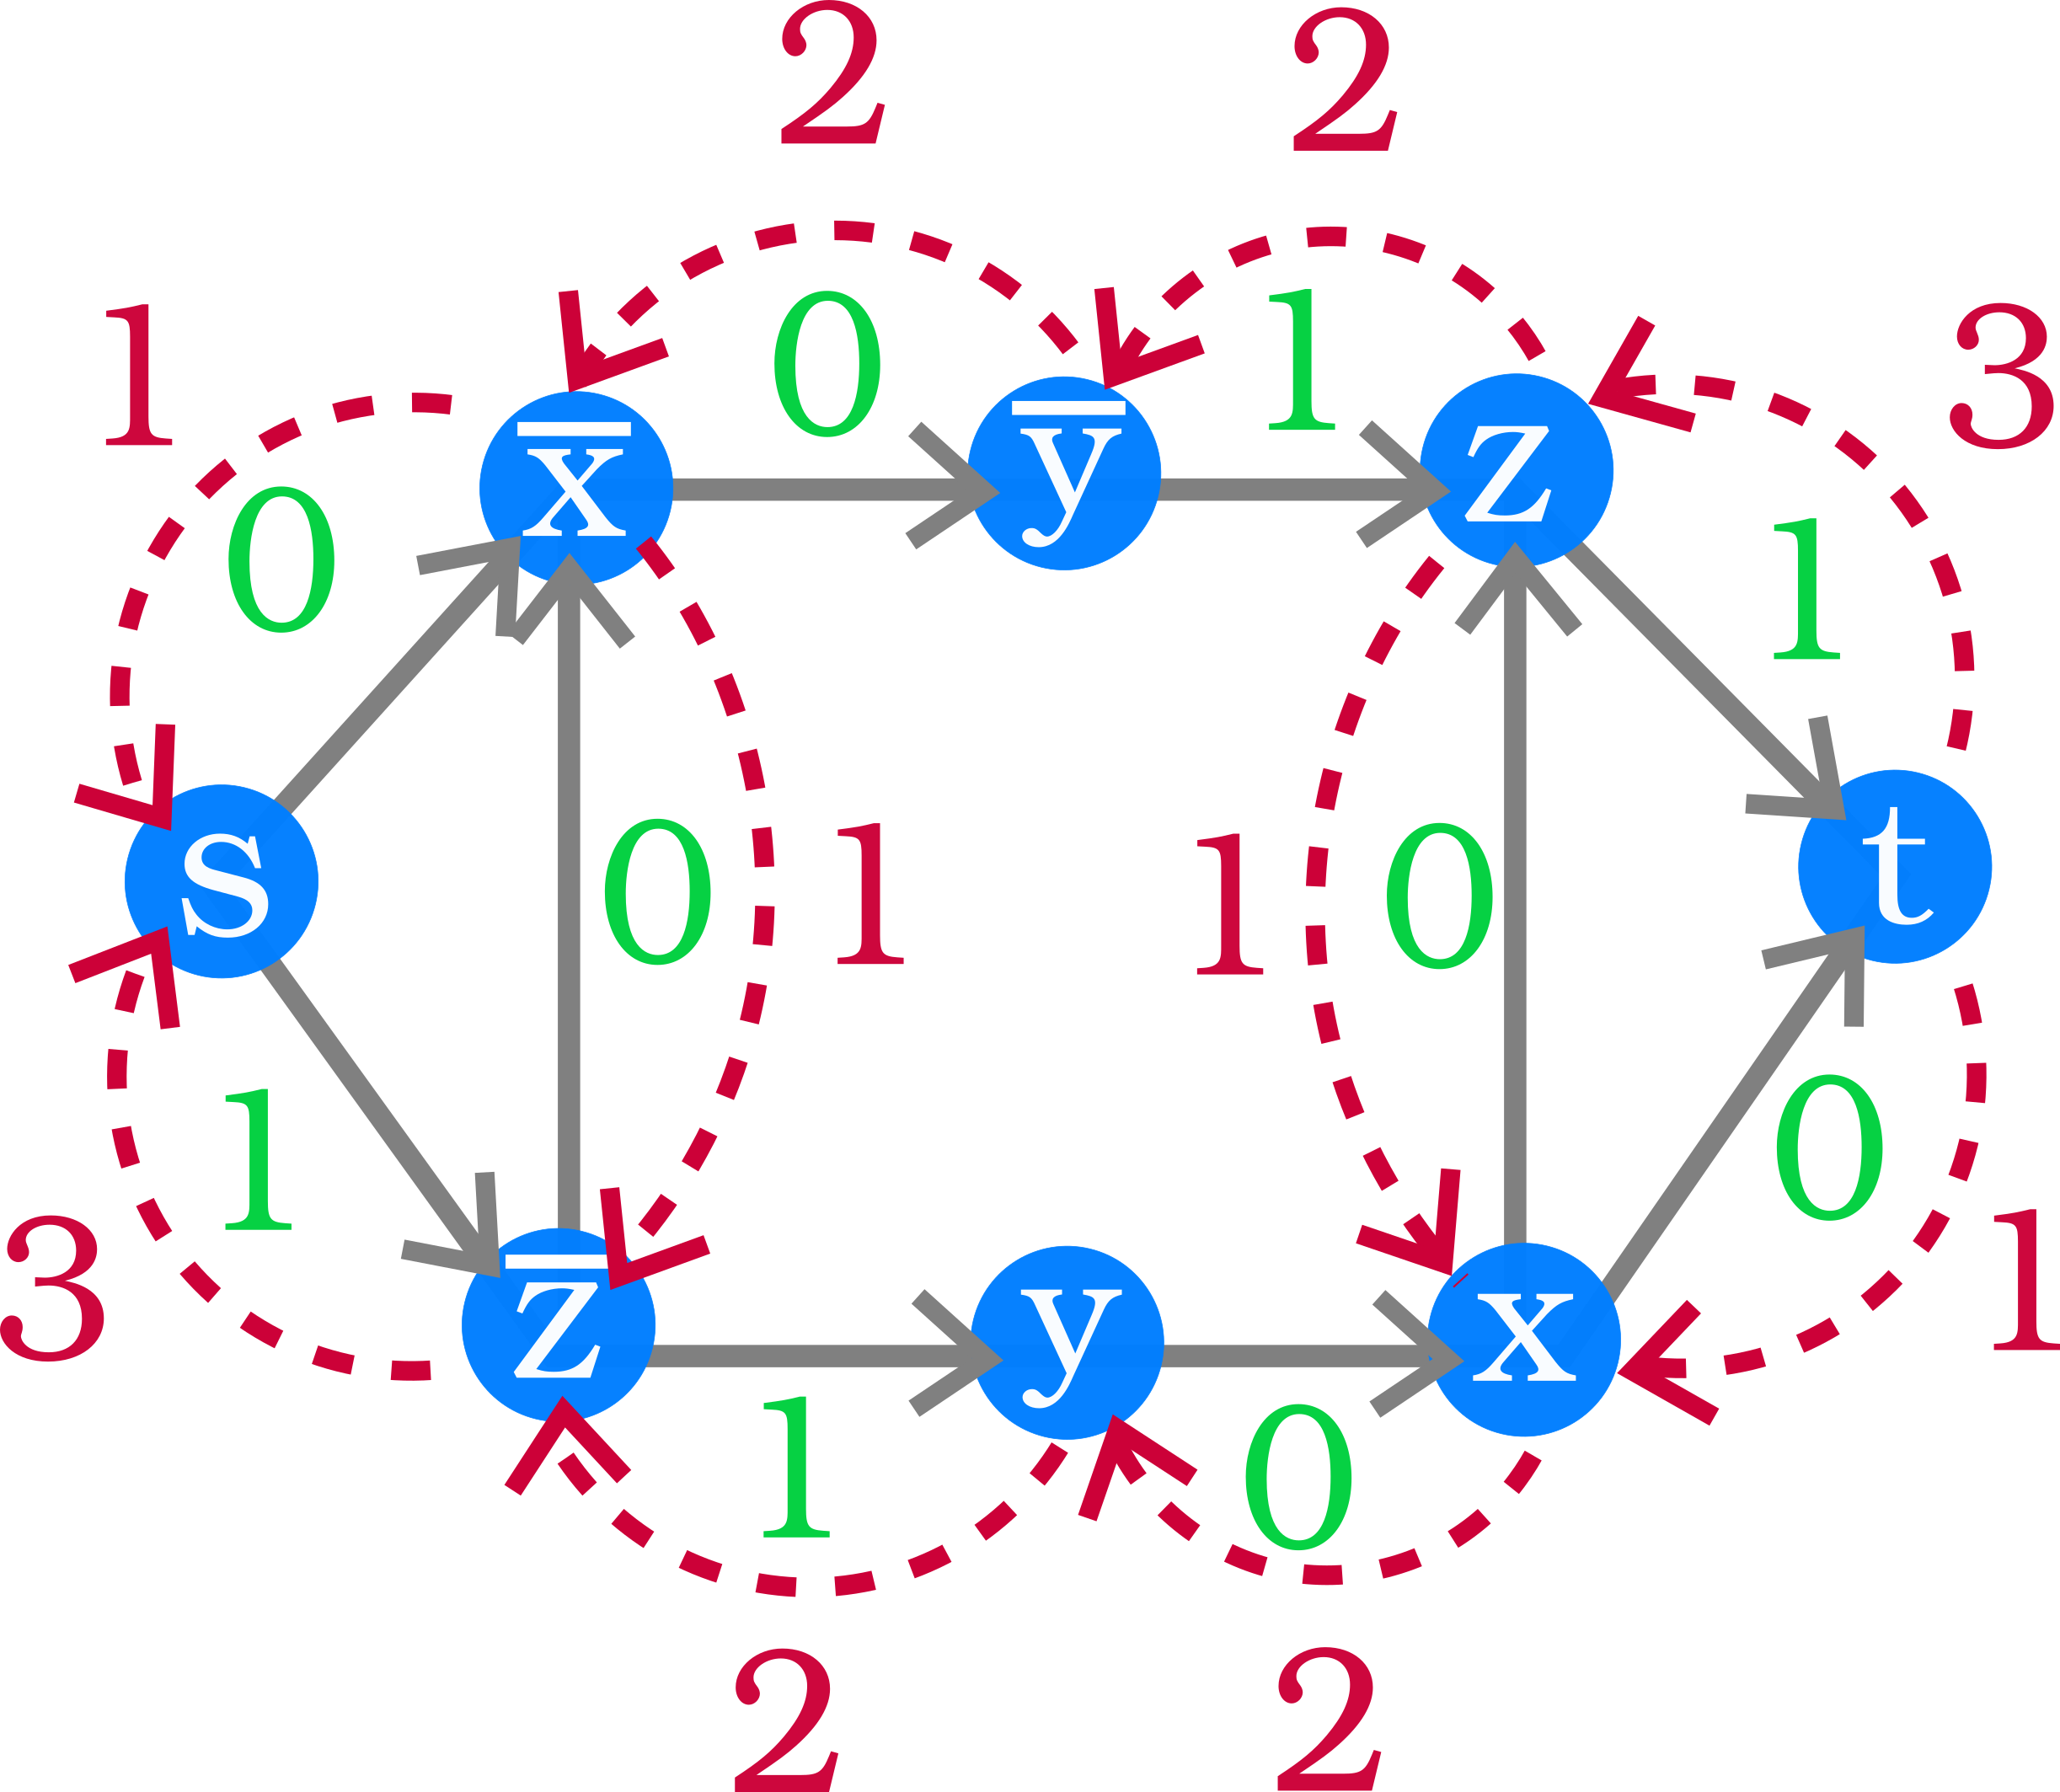
\includegraphics[scale=0.1]{figures/chapter3/posiform-graph-6.png}
}%
\caption{The Ford Fulkerson algorithm is executed for the capacitated graph representation of posiform $\phi$. In~(a), the initial capacitated graph; a sequence of augmenting paths (we omit the returning edges) are shown in figures~(b-e); the final residual graph is shown in figure~(f).  }
\label{ch2:fig:posiform-capacitated-graph}
\end{figure}

\begin{proposition}{Residual graph to posiform}
	Given a posiform 
	
	\begin{align*}
		\phi = C(\phi) + \sum_{p \in L}{a_pp} + \sum_{p,q \in L}{a_{pq}pq},
	\end{align*}
	
	construct its corresponding capacitated graph $G_{\phi}$ and compute its maximum flow executing the Ford Fulkerson algorithm. Then, for every step $k$ of the algorithm we have that
	\begin{align*}
		\phi &= C(\phi) + \nu(\varphi_k) + \phi_{ G_{ \phi [\varphi_k]}}.
	\end{align*}
\end{proposition}

\begin{proof}

We observe that every $\epsilon$-augmenting path $s,v_{p_1},v_{p_2},\cdots,v_{p_n},t$ in $G_{\phi [\varphi_k]}$ encodes an alternating sum of literals of the form

\begin{align*}
	\phi_{\pi_k} =& a_1\bar{p}_1 + a_{1\bar{2}}p_1\bar{p}_2 + a_{2\bar{3}}p_2\bar{p}_3 + \cdots + a_{n-1\bar{n}}p_{n-1}\bar{p}_k + a_np_n \\
	=&\epsilon( \bar{p}_1 + p_1\bar{p}_2 + p_2\bar{p}_3 + \cdots + p_{n-1}\bar{p}_n + p_n ) + \phi '.
\end{align*}

By observing that

\begin{align*}
	\bar{p}_1 + p_1\bar{p}_2 &= 1 - p_1p_2 \\
	-\bar{p}_{j-1}p_{j} + p_j\bar{p}_{j+1} &= \bar{p}_{j-1}p_j - p_jp_{j+1} \\
	-p_{n-1}p_n + p_n &= \bar{p}_{n-1}p_n,
\end{align*}

we can rewrite the alternating sum as

\begin{align*}
	\phi_{\pi} &= \epsilon + \epsilon( \bar{p}_1p_2 + \bar{p}_2p_3 + \cdots + \bar{p}_{n-1}p_n ) + \phi ' \\
	&= \psi + \phi ',	
\end{align*}

where

\begin{align*}
	\phi ' &= (a_{\bar{1}}-\epsilon)\bar{p}_1 + (a_{1\bar{2}} - \epsilon) p_1\bar{p}_2 + (a_{2\bar{3}}  - \epsilon)p_2\bar{p}_3 + \cdots + (a_{n-1\bar{n}} - \epsilon)p_{n-1}\bar{p}_n + (a_n -\epsilon)p_n.
\end{align*}

Note that $\phi '$ and $\psi$ corresponds, respectively, to the update of the residual costs for the edges of $\pi_k$ and its returning edges. Therefore, we can write


\begin{align*}
	\phi &= \nu(\varphi_k) + \phi_{ G_{ \phi [\varphi_k] }},
\end{align*}

i.e., the initial posiform $\phi$ can be rewritten as a constant plus the posiform corresponding to the residual graph at step $k$ of  the Ford Fulkerson algorithm. 
\end{proof}

It follows that the master posiform is given by

\begin{align*}
	\phi^{\star} &= \nu(\varphi^{\star}) + \phi_{ G_{ \phi [ \varphi^{\star}] }}.
\end{align*}

\begin{example}
The posiform $\phi = 2x + 8z + 2x\bar{z} + 4\bar{x}y + 6\bar{y}\bar{z}$ is represented by the graph $G_{\phi}$ in~\cref{ch2:fig:posiform-capacitated-graph}. Its maximum flow value  equals to $4$ and the master posiform is given by $\phi^{\star} = \nu(\varphi ^{\star}) + \phi_{G_{\phi {[\varphi^{\star}}]}} = 4 + 2z + 2\bar{z}\bar{y} + 4zy + 4\bar{y}x + 2z\bar{x}$.
\end{example}

From the strong persistency theorem we conclude that $z=0$, and we have

\begin{align*}
	\min \phi = \min \phi^{\star}(z=0) = \min 2\bar{y} + 4\bar{y}x.
\end{align*}

We can say more. Let $U$ be the set of literals that are reached from the source by a path of positive residual in the final residual graph. Then, a solution $\vec x \in \argmin f$ must agree with $x(U=1)$~\cite{boros02pseudo}. Therefore,

\begin{align*}
	\min \phi = \min \phi^{\star}(\bar{z}=1,y=1) = \min 4 = 4.
\end{align*}

In fact, by looking at all configurations of $\phi$, we observe that $(z=0,y=1)$ in every minimum configuration of $f$.

\begin{center}
\begin{tabular}{|c|c|c|c|}
\hline
$x$ & $y$ & $z$ & $f$\\
\hline
0 & 0 & 0 & 6 \\
0 & 0 & 1 & 8 \\
\textbf{0} & \textbf{1} & \textbf{0} & \textbf{4} \\
0 & 1 & 1 & 12 \\
1 & 0 & 0 & 10 \\
1 & 0 & 1 & 10 \\
\textbf{1} & \textbf{1} & \textbf{0} & \textbf{4} \\
1 & 1 & 1 & 10 \\
\hline
\end{tabular}
\end{center}

The master posiform $\phi^{\star}(f)$ gives us a lower bound for the PBF $f$, which is called the roof dual. In some fortunate occasions, the master posiform allows us to simplify the original optimization problem in a trivial one. That is the case for the class of submodular functions.

\section{Submodular functions}

\begin{definition}{Submodular set function}

Let $V$ be a set with $n$ elements, e.g., $V=\{1,2,\cdots, n\}$. A set function $f:2^V\rightarrow \mathbb{R}$ is submodular if 

\begin{align}
	f(X) + f(Y) \geq f(X \cup Y) + f(X \cap Y),\quad \forall X,Y \subset V.
	\label{ch2:eq:submodular-set-function}
\end{align}

\end{definition}

An equivalent local definition is given by

\begin{align}
	f(X \cup \{x_1\}) + f(X \cup \{x_2\}) \geq f(X \cup \{x_1,x_2\}) + f(X), \; \forall X \subset V \text{ and } \{x_1,x_2\} \not\subset X.
	\label{ch2:eq:submodular-local}
\end{align}

\begin{proposition}{Quadratic submodular PBF}
	Let $f:2^V\rightarrow \mathbb{R}$ a quadratic PBF  written as
	\begin{align*}
		f(x_1,\cdots,x_n) &= C + \sum_{i<n}{f_{i}(x_i)} + \sum_{i<j<n}{f_{ij}(x_i,x_j)}.
	\end{align*}
	Then, the statements below are equivalent
	\begin{itemize}
	 	\item[i]{Function $f$ is submodular.}
		\item[ii]{ $f_{ij}(0,0) + f_{ij}(1,1) \leq f_{ij}(0,1) + f_{ij}(1,0), \quad \forall i<j<n$}
		\item[iii]{ $\frac{\partial^2 f}{\partial x_i\partial x_j} \leq 0, \quad \forall i<j<n$ }
	\end{itemize}
	\begin{proof}
	
	\begin{tabular}{rl}
	$\mathbf{(i\rightarrow ii)}$:& Immediately from~\cref{ch2:eq:submodular-local}. \\	
	$\mathbf{(ii\rightarrow iii)}$:&  Writing down the terms in $f$ for variables $x_i,x_j$ we have
	\end{tabular}
	
	\begin{align*}
		f_{ij}(0,0)(1-x_i)(1-x_j) + f_{ij}(1,1)x_ix_j + f_{ij}(0,1)(1-x_i)x_j + f_{ij}(1,0)x_i(1-x_j).
	\end{align*}

	Taking its second derivative

	\begin{align*}
		\frac{\partial^2f}{\partial x_i\partial x_j} &= f_{ij}(0,0) + f_{ij}(1,1) - f_{ij}(0,1) - f_{ij}(1,0)
	\end{align*}
	
	\begin{tabular}{rl}
		$\mathbf{(iii\rightarrow i)}$:& We define
	\end{tabular}		
	
		\begin{align*}
			\Delta_{x_i} &= f(x_1,\cdots,x_{i-1},x_i=1,x_{i+1},\cdots,x_n) - f(x_1,\cdots,x_{i-1},x_i=0,x_{i+1},\cdots,x_n) \\
			&= f(X \cup \{x_i\}) - f(X), \quad \text{ where } x_i \notin X.
		\end{align*}		 		
		Therefore
		\begin{align*}
			f( X \cup \{x_1,x_2\}) &= f(X) + \Delta_{x_1} + \Delta_{x_2} + \frac{ \partial^2 f}{\partial x_i \partial x_j} \\
			f( X \cup \{x_1,x_2\}) &= -f(X) + f(X \cup \{x_1\}) + f(X \cup \{x_2\}) + \frac{ \partial^2 f}{\partial x_i \partial x_j}.
		\end{align*}	
		
		Finally,
		\begin{align*}
			f( X \cup \{x_1,x_2\}) +f(X) - f(X \cup \{x_1\}) - f(X \cup \{x_2\}) &\leq 0.	
		\end{align*}
		
	\end{proof}
\end{proposition}





\section{Graph-cut models}

%\subsection{Hidden Markov Model}
%\subsection{Potts and Ising model}
%\section{Pseudo-Boolean functions}
%\subsection{Definition, properties, subclasses}
%\subsection{Algorithms: general submodular, quadratic submodular (graph-cut), other classes, roof-duality }
%\section{GraphCut}
%\subsection{Submodular to graph-cut}
%\subsection{Grabcut}
%\subsection{alpha expansion, alfa-beta swap}
%\section{Image denoising}
%\section{Image segmentation}
%	\subsection{Graph-cuts}
%	\subsection{Watersheds}
%	\subsection{Morphology}	
%	\subsection{Thresholding}		
%	\subsection{Wavelets}		
%	\subsection{Corner, edge detection, filters}
%	\subsection{Region adjacenty graph}
%	\subsection{K-means segmentation}	
%	\subsection{Hough transform, parameter space}
%\section{Image inpainting}	